% Template for PLoS
% Version 3.5 March 2018
%
% % % % % % % % % % % % % % % % % % % % % %
%
% -- IMPORTANT NOTE
%
% This template contains comments intended 
% to minimize problems and delays during our production 
% process. Please follow the template instructions
% whenever possible.
%
% % % % % % % % % % % % % % % % % % % % % % % 
%
% Once your paper is accepted for publication, 
% PLEASE REMOVE ALL TRACKED CHANGES in this file 
% and leave only the final text of your manuscript. 
% PLOS recommends the use of latexdiff to track changes during review, as this will help to maintain a clean tex file.
% Visit https://www.ctan.org/pkg/latexdiff?lang=en for info or contact us at latex@plos.org.
%
%
% There are no restrictions on package use within the LaTeX files except that 
% no packages listed in the template may be deleted.
%
% Please do not include colors or graphics in the text.
%
% The manuscript LaTeX source should be contained within a single file (do not use \input, \externaldocument, or similar commands).
%
% % % % % % % % % % % % % % % % % % % % % % %
%
% -- FIGURES AND TABLES
%
% Please include tables/figure captions directly after the paragraph where they are first cited in the text.
%
% DO NOT INCLUDE GRAPHICS IN YOUR MANUSCRIPT
% - Figures should be uploaded separately from your manuscript file. 
% - Figures generated using LaTeX should be extracted and removed from the PDF before submission. 
% - Figures containing multiple panels/subfigures must be combined into one image file before submission.
% For figure citations, please use "Fig" instead of "Figure".
% See http://journals.plos.org/plosone/s/figures for PLOS figure guidelines.
%
% Tables should be cell-based and may not contain:
% - spacing/line breaks within cells to alter layout or alignment
% - do not nest tabular environments (no tabular environments within tabular environments)
% - no graphics or colored text (cell background color/shading OK)
% See http://journals.plos.org/plosone/s/tables for table guidelines.
%
% For tables that exceed the width of the text column, use the adjustwidth environment as illustrated in the example table in text below.
%
% % % % % % % % % % % % % % % % % % % % % % % %
%
% -- EQUATIONS, MATH SYMBOLS, SUBSCRIPTS, AND SUPERSCRIPTS
%
% IMPORTANT
% Below are a few tips to help format your equations and other special characters according to our specifications. For more tips to help reduce the possibility of formatting errors during conversion, please see our LaTeX guidelines at http://journals.plos.org/plosone/s/latex
%
% For inline equations, please be sure to include all portions of an equation in the math environment.  For example, x$^2$ is incorrect; this should be formatted as $x^2$ (or $\mathrm{x}^2$ if the romanized font is desired).
%
% Do not include text that is not math in the math environment. For example, CO2 should be written as CO\textsubscript{2} instead of CO$_2$.
%
% Please add line breaks to long display equations when possible in order to fit size of the column. 
%
% For inline equations, please do not include punctuation (commas, etc) within the math environment unless this is part of the equation.
%
% When adding superscript or subscripts outside of brackets/braces, please group using {}.  For example, change "[U(D,E,\gamma)]^2" to "{[U(D,E,\gamma)]}^2". 
%
% Do not use \cal for caligraphic font.  Instead, use \mathcal{}
%
% % % % % % % % % % % % % % % % % % % % % % % % 
%
% Please contact latex@plos.org with any questions.
%
% % % % % % % % % % % % % % % % % % % % % % % %

\documentclass[10pt,letterpaper]{article}
\usepackage[top=0.85in,left=2.75in,footskip=0.75in]{geometry}

\usepackage{amsmath,amssymb}
\usepackage{changepage}
\usepackage[utf8x]{inputenc}
\usepackage{textcomp,marvosym}
\usepackage{cite}
\usepackage{nameref,hyperref}
\usepackage[right]{lineno}
\usepackage{microtype}
\DisableLigatures[f]{encoding = *, family = * }
\usepackage[table]{xcolor} 
\usepackage{array}
\newcolumntype{+}{!{\vrule width 2pt}}
% create \thickcline for thick horizontal lines of variable length
\newlength\savedwidth
\newcommand\thickcline[1]{%
  \noalign{\global\savedwidth\arrayrulewidth\global\arrayrulewidth 2pt}%
  \cline{#1}%
  \noalign{\vskip\arrayrulewidth}%
  \noalign{\global\arrayrulewidth\savedwidth}%
}
% \thickhline command for thick horizontal lines that span the table
\newcommand\thickhline{\noalign{\global\savedwidth\arrayrulewidth\global\arrayrulewidth 2pt}%
\hline
\noalign{\global\arrayrulewidth\savedwidth}}

% Remove comment for double spacing
%\usepackage{setspace} 
%\doublespacing

% Text layout
\raggedright
\setlength{\parindent}{0.5cm}
\textwidth 5.25in 
\textheight 8.75in

% Bold the 'Figure #' in the caption and separate it from the title/caption with a period
% Captions will be left justified
\usepackage[aboveskip=1pt,labelfont=bf,labelsep=period,justification=raggedright,singlelinecheck=off]{caption}
\renewcommand{\figurename}{Fig}

% Use the PLoS provided BiBTeX style
\bibliographystyle{plos2015}

% Remove brackets from numbering in List of References
\makeatletter
\renewcommand{\@biblabel}[1]{\quad#1.}
\makeatother

% Header and Footer with logo
\usepackage{lastpage,fancyhdr,graphicx}
\usepackage{epstopdf}
%\pagestyle{myheadings}
\pagestyle{fancy}
\fancyhf{}
%\setlength{\headheight}{27.023pt}
%\lhead{\includegraphics[width=2.0in]{PLOS-submission.eps}}
\rfoot{\thepage/\pageref{LastPage}}
\renewcommand{\headrulewidth}{0pt}
\renewcommand{\footrule}{\hrule height 2pt \vspace{2mm}}
\fancyheadoffset[L]{2.25in}
\fancyfootoffset[L]{2.25in}
\lfoot{\today}

%% Include all macros below
\newcommand{\lorem}{{\bf LOREM}}
\newcommand{\ipsum}{{\bf IPSUM}}
%% END MACROS SECTION


\begin{document}
\vspace*{0.2in}

% Title must be 250 characters or less.
\begin{flushleft}
{\Large
\textbf\newline{Evaluating Uniform Sampling Methods for Flux Balance Analysis} % Please use "sentence case" for title and headings (capitalize only the first word in a title (or heading), the first word in a subtitle (or subheading), and any proper nouns).
}
\newline
\\
Lucy Vass\textsuperscript{1\textcurrency}, %\Yinyang
Helena Herrmann\textsuperscript{2}, %\Yinyang
Jean-Marc Schwartz\textsuperscript{2},
\\
\bigskip
\textbf{1} Faculty of Biology, Medicine and Health, The University of Manchester, Manchester, Greater Manchester, United Kingdom
\\
\textbf{2} Faculty of Science and Engineering, The University of Manchester, Manchester, Greater Manchester, United Kingdom
\\
\bigskip

% Primary Equal Contribution Note
%\Yinyang These authors contributed equally to this work.

% Additional Equal Contribution Note
% Also use this double-dagger symbol for special authorship notes, such as senior authorship.

% Current address notes
\textcurrency Current Address: %Insert University of Bristol info in the above format 

% change symbol to "\textcurrency a" if more than one current address note

% Use the asterisk to denote corresponding authorship and provide email address in note below.
* Jean-marc.Schwartz@manchester.ac.uk

\end{flushleft}
% Please keep the abstract below 300 words
\section*{Abstract}
Flux balance analysis (FBA) and Flux Variability Analysis (FVA) are a powerful techniques for probing constraint-based, genome-scale metabolic reconstructions, but the analyses are limited to reporting single values or the minimum and maximum flux values. Uniform samplers, based on Monte Carlo Markov chain methods, however, allow the elucidation of the underlying flux probability distributions of reactions in the metabolic reconstruction.

Here, we evaluate the performance of three modern uniform samplers available in the COBRA Toolbox and COBRApy package; CHRR, ACHR and OPTGP. Using models with a flux solution space up to 130 dimensions, we show that CHRR converges to a stationary uniform distribution in the fewest sampling steps, and that this is not affected by the dimensionality of the flux solution space. However, we find that CHRR run time per sampling step is up to 20 times slower than OPTGP, which can make CHRR impractical for sampling very high dimension models. A comparison of the flux probability distributions produced by each sampler showed there is very little difference between the samples produced, but that in some reactions, CHRR showed a slight bias towards extreme flux values.

To demonstrate the utility of uniform flux sampling, the OPTPG sampler was used to compare the flux probability distributions of a metabolic breast cancer model and a healthy breast cell model. We then used a \textit{Arabidopsis thaliana} leaf metabolic model to analyze the differences of optimal and near-optimal biomass production on flux distributions. Both set-ups effectively demonstrate how traditional FBA and FVA can fail to capture biologically meaningful system properties. 

% Please keep the Author Summary between 150 and 200 words
% Use first person. PLOS ONE authors please skip this step. 
% Author Summary not valid for PLOS ONE submissions.

\section*{Author summary} 
The current era of high-throughput data generating technologies and the availability of many genome-scale metabolic models for all model organisms require efficient and accurate methods of analysis which can be used to understand the available biological data in as much detail as possible. 

While Flux Balance Ananlysis (FBA) and Flux Variability Analysis (FVA) are the current methods of choice for analyzing large metabolic networks, they fail to capture the underlying flux distributions which quantify the total feasible flux space of individual reactions under given conditions. Flux sampling methods, which generate flux probability distributions of metabolic reactions, provide an elegant solutions to understanding the total feasible flux space. 

We analyze the current most popular solutions for flux sampling and compare them to one another, in order to provide computational biologists with guidelines for which methods are most appropriate for their analyses. To extent of our knowledge the convergence, run-time and scalability of the CHRR, ACHR and OPTGP sampling algorithms as implemented in the COBRA toolbox and COBRApy have not yet been directly compared in the context of metabolic modelling. 

Here we demonstrate that analyzing the total feasible flux space using an appropriate sampling algorithm can provide valuable biological information when comparing cancerogenic to healthy metabolisms and when comparing optimal to near-optimal biomass production in plants. 


\linenumbers

\section*{Introduction}

\subsection*{Genome-scale metabolic reconstructions}
Over the last decade, modern high-throughput genome-sequencing technologies have enabled a rapid increase in the number of genome-scale metabolic reconstructions. Since the completion of the first genome-scale metabolic reconstruction of \textit{Haemophilus influenzae} almost 20 years ago\cite{Edwards}, reconstructions of 113 bacteria and 57 eukaryota have been produced and validated\cite{Adam}. These reconstructions have enabled systems biologists to investigate metabolism at a cellular level, providing advancements in a variety of fields including bioengineering, host-pathogen relationships and plant biology. 

Genome-scale metabolic reconstructions combine gene functional annotations and biochemical pathways, ultimately linking genotype to phenotype. This is mainly achieved through gene sequence alignment between annotated and unannotated genes, pathway databases (for example KEGG\cite{kegg}) and primary literature searches \cite{Oberhardt}. To utilise the information in these reconstructions, two approaches are most commonly used; kinetic analysis and constraint-based analysis. Kinetic analysis of genome-scale metabolic reconstructions is challenging due to the lack of available and accurate kinetic parameter measurements of the enzymes in the network. These must be derived from experimental data which can be time consuming to collect and has the potential to be inaccurate \cite{Orth}. The alternative, constraint-based analysis, imposes a steady-state constraint of the flow of metabolites through each reaction in the model. These constraints can be defined through various means including the mass balance of reactions (stoichiometric coefficients), thermodynamics or fluxomics (using 13\textsuperscript{C} to track metabolite concentrations)\cite{Ebrahim}.

\subsection*{Flux balance and flux variability analysis}
The most popular method of analyzing constraint-based models is flux balance analysis (FBA). In this approach the rate, or flux, of each reaction in the network is constrained by its stoichiometric coefficients. Stoichiometric coefficients are the ratio of reactants and their constituent molecules. These stoichiometric coefficients can be represented as a matrix of reactions against metabolites, effectively turning the network into a series of mathematical equations which define a finite flux solution space\cite{Orth}. This solution space defines all the potential metabolic phenotypes which can occur in the organism at a steady-state\cite{Wiback}. 
To assess metabolism of different phenotypes or conditions, FVA requires an objective function to be specified which represents the metabolic aim of the cell at steady-state. A biologically relevant objective function is often created and added to the network as an artificial reaction. A common objective function in FBA is biomass production, which can be used to calculate growth rate. The biomass objective function sums the metabolite content of essential macromolecules, such as proteins and lipids and then is added to the model as an output reaction\cite{Feist}. FBA then uses linear programming algorithms to compute the resulting flux through all the reactions in the network such that biomass production is maximized\cite{Orth}. 

FBA has been used for a variety of applications in synthetic biology. For example, prediction of metabolites yields under different environmental conditions. In one such study, FBA was used to simulate the effects of changing nitrogen source on the energy cost of protein synthesis\cite{Arnold}. Alternatively, FBA has been used to assess the impact of gene knockouts \textit{in silico}, for example in microbiology to elucidate the enzymes \textit{M. tuberculosis} uses to evade the immune system\cite{Bose}. Another application is in bioengineering, such as in one study where FBA was combined with wet-lab validation to discover pathways to produce a drug molecule in \textit{E. coli}\cite{Immanuel}. Finally, FBA has played a role in expanding and validating genome-scale metabolic reconstructions, where it has been used to fill knowledge gaps\cite{Karp} and identify redundant or linked metabolic pathways\cite{Papin}.

In most cases, FBA's user-friendly ability to accommodate for complexity and little requirement for experimental data, consequently results in non-unique flux distributions \cite{antoniewicz} such that many single point solutions exists and are at random returned by FBA. Mathematically, this technicality can be overcome by either analyzing the whole range of possible fluxes using Flux Variability Analysis (FVA) or by implementing additional objectives which further constrain the flux space. In order to avoid non-linear programming, multiple objective functions are often introduced as a hierarchy, whereby a secondary objective is imposed after setting the primary objective to its calculated, optimal flux value. Otherwise, in order to quantify how one objective can be made only at the cost of another, the Pareto surface should be analyzed\cite{schuetz}. Flux Variability Analysis (FVA) returns the upper and lower most feasible values as computed by FBA, thus indicating the flux bounds of the total feasible solution space. Notably, FVA only gives the range of the solution space for each reaction in the metabolic model and provides no indication as to which single-point solutions are most likely or whether all single point solutions within the bounds exist. 

Studying the shape and volume of the complete steady-state solution space can allow more in-depth insights into a model because this information can be used to determine the likelihood of varying flux values. For example, metabolic redundancies and subtle metabolic differences which results in an identical phenotype are captured in the shape of the solution space. This information can be obtained by using mathematical techniques such as convex analysis and vertex enumeration, which give the exact properties and volume of the solution space\cite{Schellenberger}. However, due to their computational intensiveness, these methods are only efficient when applied to small, simple networks\cite{Wiback}. In contrast, genome-scale metabolic reconstructions are complex and consist of many reactions, creating highly dimensional, irregularly shaped solution spaces. An alternative approach to study the solution space of these networks is to use uniform sampling\cite{Schellenberger}.

\subsection*{Uniform sampling of the solution space}
An effective way to study the flux steady-state solution space is through random sampling. This approach has been used successfully in a range of fields and gives a deeper understanding of the metabolic network. For example, sampling has been used to design wet-lab experiments to detect enzymopathies\cite{Price} and to understand transcriptional regulation of metabolites\cite{Bordel}.

Monte Carlo algorithms are a class of algorithms which use random sampling to estimate the solution to deterministic problems\cite{Harrison} and the method of choice for studying the flux solution space. A simple Monte Carlo method, also known as rejection sampling, produces random points and calculates the fraction of those which landed within the constraints of the solution space\cite{Wiback}. To understand this method, it can be applied to a simple problem such as estimating the value of $\pi$ \textbf{(Fig \ref{figure:1}A)}. First, a random number generator is used to produce points within a grid of Cartesian coordinates which contain a quarter of a circle. The coordinates lie within the area of the circle if they are less than the circle’s radius in distance away from the origin (0,0). The fraction of points within (accepted) and outside (rejected) the circles bounds can then be used to estimate the area and therefore $\pi$. The larger the number of points in the sample, the more accurate the estimation of $\pi$\cite{MCpi}.

\begin{figure}[!h]
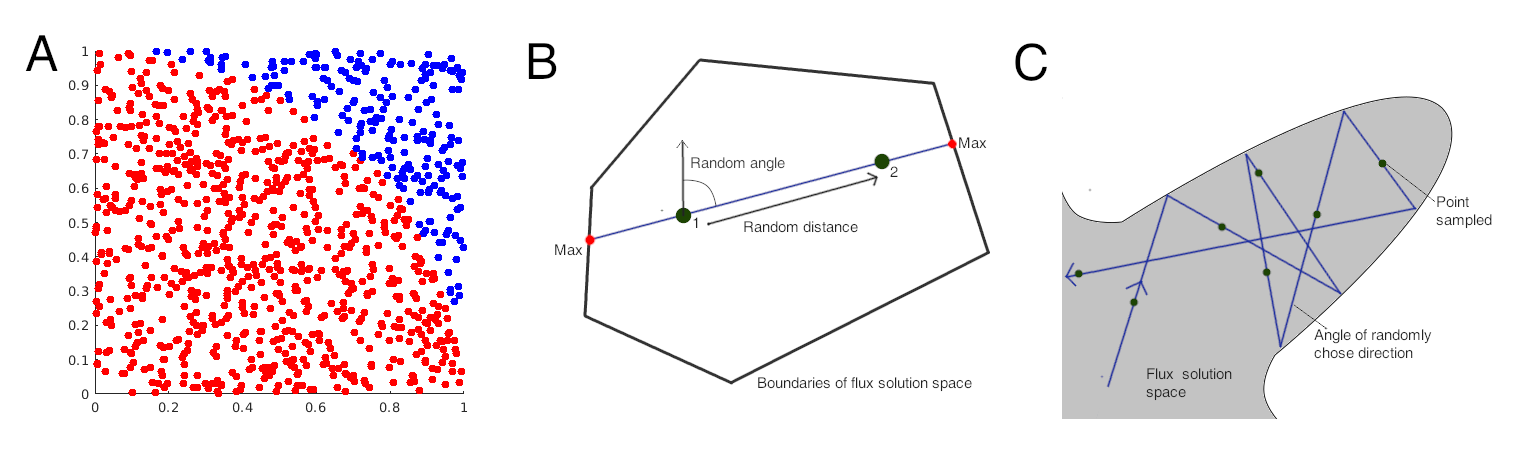
\includegraphics[scale=1]{fig1.png}
\caption{{\bf Monte Carlo sampling and the hit-and-run algorithm.} \\
A) Estimating the value of $\pi$ by Monte Carlo sampling and a grid of cartesian coordinates. $\pi ={number\,of\,accepted\,samples\,(red)} \ {total\,number\,of\,samples\,(blue)} \cdot 4$ \\
B) Direction and distance choice of each step of the hit-and-run algorithm. Adapted from Megchelenbrink \textit{et al}. (2014)\cite{Megchelenbrink}. \\
C) Trapping of the hit-and-run algorithm in elongated boundaries of the hit-and-run algorithm.\\}
\label{figure:1}
\end{figure}

In relation to constraint-based metabolic models, Monte Carlo methods can produce a series of random points which conform to the constraints of the model. These points represent a uniform sample of the flux values within the solution space, therefore providing an estimate of the probability density function of each reaction in the model\cite{Wiback}. The probability density function describes the likelihood of all possible flux rates through the reaction. As with the example of estimating $\pi$, the sample must both be uniformly distributed and sufficiently large to give an accurate estimation.

Monte Carlo methods therefore seem to provide an elegant solution to the problem of studying the complex solution space. However, when sampling highly-dimensional solution spaces, this method is very inefficient. Wiback \textit{et al}. (2004) implemented Monte Carlo sampling to study the solution space of an human erythrocyte metabolic model and found that only 1 in 5,000 randomly generated points fell within the constraints of the model\cite{Wiback}. This is because the search space, or ‘bounding box’ of the solution space is too large in volume in comparison to the solution space, leading to a high rate of points falling outside the constraints. There are two options to overcoming this; further constraining the bounding box, or ensuring samples are only drawn from within the solution space. .. 
 
\subsubsection*{Hit-and-run}
The hit-and-run algorithm, more formally known as a Markov Chain Monte Carlo (MCMC), has numerous applications in science, from Bayesian statistics to psychology\cite{Ravenzwaaij}. Hit-and-run algorithms overcome the inefficiency of basic Monte Carlo sampling methods by only sampling directly within the solution space\cite{Kiatsupaibul}. These algorithms add an additional property to Monte Carlo sampling; Markov chains. This property means that samples are generated in a sequence, using information from the previous point to generate the current point\cite{Ravenzwaaij}. The Markovian nature of hit-and-run insures that the sample created will uniformly cover a convex solution space in a finite amount of point draws, or steps\cite{Ravenzwaaij}.

The name ‘hit-and-run’ describes how the algorithm moves around and explores the solution space \textbf{(Fig \ref{figure:1}B)}. On the first iteration of the algorithm, the starting point on the boundary of the solution space is found. After that, each ‘step’ of the algorithm consists of three stages as described by Kaufman \textit{et al.} (1994):
\begin{enumerate}
\item from the current point, a direction is randomly chosen; there is equal probability that any direction will be chosen,
\item the sampler moves a random distance in the chosen direction. The maximum distance is the boundary of the solution space, 
\item the point it lands on is added to the sample. 
\end{enumerate}
% If we need to reduce content could possibly cut down these explanations here

Whilst hit-and-run algorithms provide an efficiency advantage to basic Monte Carlo methods, it can still take a large number of steps to produce a uniform sample of complex solution spaces. It’s possible that in elongated, irregular solution spaces, such as those often produced by FBA, that the hit-and-run algorithm can become ‘trapped’ in areas of the solution space near the boundaries\cite{Megchelenbrink}\cite{Hogg}\textbf{(Fig \ref{figure:1}C)}. This could lead to an increased density of samples being drawn from these areas and additionally prevent the algorithm from fully sampling the whole solution space within a practical number of steps\cite{Hogg}.

\subsubsection*{The importance of convergence}
Convergence is achieved when the sample has reached the target distribution. In the context of sampling the flux solution space, this is the number of samples needed to produce a uniform sample across the entire solution space. When convergence is achieved, the sample is an accurate representation of the actual solution space\cite{Hamra}. Precisely defining convergence is difficult because we don’t know the exact nature of the solution space. Therefore, convergence has to be assumed when there is no evidence of non-convergence \cite{Hamra}. The key factor which affects the convergence is the length of the hit-and-run sampling chains. To create a uniform sample, and therefore an accurate estimation of the probability density function for each reaction, the chains produced by hit-and-run samplers must be long enough to fully explore the solution space. At convergence, the probability distribution of the sample will become stationary. This means that no matter how many more steps of the sampler are run, the probability density function remains the same\cite{Hamra}. At convergence, the descriptors of the sample such as the median, mean, IQR and range should stay constant, and large fluctuations of these are evidence of non-convergence. Non-convergence could lead to incorrect conclusions about the network.

The Markovian nature of the hit-and-run sampler guarantees that it will converge in a finite number of steps\cite{Ravenzwaaij}. However, due to the problems of edge trapping, hit-and-run samplers can take an impractically large number of steps to reach convergence\cite{Megchelenbrink}. Modern hit-and-run samplers for use in FBA have been developed to overcome this limitation and reduce the number of steps needed to produce a uniform sample which fully represents the probability density function.

\subsection*{COBRA Toolbox}
The COBRA (Constraint-based reconstruction and analysis toolbox) Toolbox, first released in 2007, is one of the most popular and powerful software packages for building and analysing constraint-based metabolic models\cite{Schellenberger2011}. The COBRA Toolbox is a MATLAB package that provides a suite of methods including visualisation of metabolic networks, tools for \textit{in silico} gene knockouts, fluxomics and FBA. Models can be input and output using SMBL (Systems Biology Markup Language), allowing integration with other systems biology pipelines and metabolic network databases\cite{Schellenberger2011}.

COBRApy is an open-source community Python project. The aims of the project were to to provide the features of the COBRA Toolbox non-commercially and to allow integration of more different data sources, such as transcriptomics data, into constraint-based models. Additionally, COBRApy supports parallel processing, improving run time of computationally intensive methods such as Monte Carlo sampling\cite{Ebrahim}.

Both COBRA Toolbox and COBRApy offer multiple Monte Carlo algorithms for uniform sampling of the FBA solution space\cite{Schellenberger2011}\cite{Ebrahim}. The three most modern and best performing algorithms available are: Artificially centred hit-and-run (ACHR), Optimised general parallel sampler (OPTGP) and Coordinate hit-and-run with rounding (CHRR) \textbf{(Table \ref{table:1})}.

%Why are we analysing these three algorithms and what are their uses 

\begin{table}[ht!]
\begin{adjustwidth}{-2.25in}{0in}
\centering
\caption{
{\bf Comparison of three modern algorithms for sampling constraint-based models available in the COBRA toolbox and COBRAPy package.}}
%\begin{tabular}{|c|l|l|l|l|}
\begin{tabular}{|>{\raggedright}p{2cm}>{\raggedright\arraybackslash}p{3cm}>{\raggedright\arraybackslash}p{5cm}>{\raggedright\arraybackslash}p{5cm}>{\raggedright\arraybackslash}p{2cm}|}
\hline
%\multicolumn{4}{|l|}{\bf Heading1} & \multicolumn{4}{|l|}{\bf Heading2}\\ \thickhline
\textbf{Sampler name} & \textbf{First published} & \textbf{Key features} & \textbf{Performance comparison} & \textbf{Availability in COBRA} \\
\hline\hline
\textbf{ACHR} & Kaufman \textit{et al}. (1994)\cite{Kaufman} & Estimates the centre of the solution space at each step and uses this to bias the direction choice of the algorithm. & Shown to converge in fewer steps the hit-and-run algorithm in Kaufman \textit{et al}. (1994)\cite{Kaufman}. & Python and MATLAB \\
\hline
\textbf{OPTGP} & Megchelenbrink \textit{et al}. (2014)\cite{Megchelenbrink} & Uses the solution space boundaries to generate warm-up points. Sampling based on ACHR. Uses parallel programming to run multiple short chains. & Shown to produce more samples in a faster run time and converge at lower sample sizes than the generalised parallel sampler in Megchelenbrink \textit{et al}. (2014)\cite{Megchelenbrink}. & Python \\
\hline
\textbf{CHRR} & Haraldsdottir \textit{et al}. (2017)\cite{Haraldsdottir} & A preprocessing step rounds the solution space into an ellipsoid and transforms it into a unit ball. & Shown to converge several times faster than ACHR and with shorter run times per step in Haraldsdottir \textit{et al}. (2017)\cite{Haraldsdottir}. & MATLAB\\
\hline
\end{tabular}
\label{table:1}
\end{adjustwidth}
\end{table}

\subsubsection*{Artificially centred hit-and-run (ACHR)}
To overcome the edge trapping problems of the hit-and-run sampler, Kaufman \textit{et al}. (1994) developed a method for generating the direction of movement in each step to be biased towards the centre of the solution space, therefore directing the sampler away from edges of the model\cite{Kaufman}. To begin, the algorithm performs a ‘warm-up’ stage to find initial points within the solution space and uses these to estimate the centre of the solution space. Then, the main sampling phase begins and after each point is sampled, the estimate of the centre of the solution space is revised. This is used to inform the weighting of the random direction choice. 

The artificial centreing of the algorithm increases the maximum distance the sampler is able to travel away from the previous point, allowing the algorithm to traverse throughout the space in fewer steps than conventional hit-and-run samplers. However, in implementing the artificial centering, the Markovian nature of the sampler is lost; the choice of the next point is influenced by all the points in the sequence before it, as these were used to estimate the centre. Due to this, there is no longer a guarantee that ACHR will reach convergence at a stationary, uniform sample in a finite amount of steps. However, due to its ability to explore the solution space more quickly, convergence is likely to be greatly accelerated in comparison to the hit-and-run sampler\cite{Kaufman}.

\subsubsection*{Optimised general parallel sampler (OPTGP)}
The optimized general parallel sampler (OPTGP), described in Megchelenbrink \textit{et al}. (2014), is based on ACHR and is an improvement on the widely used generalised parallel sampler\cite{Schellenberger2011}\cite{Megchelenbrink}. In the samplers warm-up phase, linear programing is used to find the minimum and maximum flux rate of each reaction. This gives twice as many warm-up points as there are reactions and these points lie on the boundaries of the flux solution space. In the sampling phase of the algorithm, ACHR is used to move around the sampling space. However, the OPTGP algorithm differs from ACHR in two ways. Firstly, from the warm-up point it produces a short chain and then only adds the last point in the chain to the sample. This gives the sampler opportunity to move away from the warm-up points and better explore the solution space. This sampled point is then used as a warm-up point for the next chain. Second, the algorithm utilises parallel programming, using the multiple processors of the computer to run multiple sampling chains in parallel. This allows larger samples to be generated in shorter run times\cite{Megchelenbrink}. OPTGP has been shown to be an improvement on the generalised parallel sampler, but has not been directly compared to ACHR.


\subsubsection*{Coordinate hit-and-run with rounding (CHRR)}
CHRR begins with a preprocessing step which aims to transform the flux solution space into a more regular, convex shape\cite{Haraldsdottir}. Doing so will prevent edge trapping and allow the sampler to traverse the space efficiently. Algorithms such as the hit-and-run algorithm have been proven to converge in around $On^{3}$ steps when sampling a regular convex body\cite{Lovasz}. Haraldsdottir \textit{et al}. (2017) developed an efficient method of rounding the irregular, highly dimensional flux solution space by calculating the maximum volume inscribed ellipsoid of the solution space \textbf{(Fig \ref{figure:2})}\cite{Haraldsdottir}. This ellipsoid is then transformed into a unit ball, or sphere with dimensions of one unit. Sampling is then carried out by using a hit-and-run sampler to move around the coordinates of the transformed solution space. At the end of sampling, the solution space transformation is reversed to obtain the original value of the sampled points\cite{Haraldsdottir}. Experimentally, CHRR has been shown to converge in up to 730 times fewer steps than ACHR\cite{Haraldsdottir}. However, this comparison relied on only one measure of convergence. CHRR has not yet been directly compared to OPTGP.

\begin{figure}
	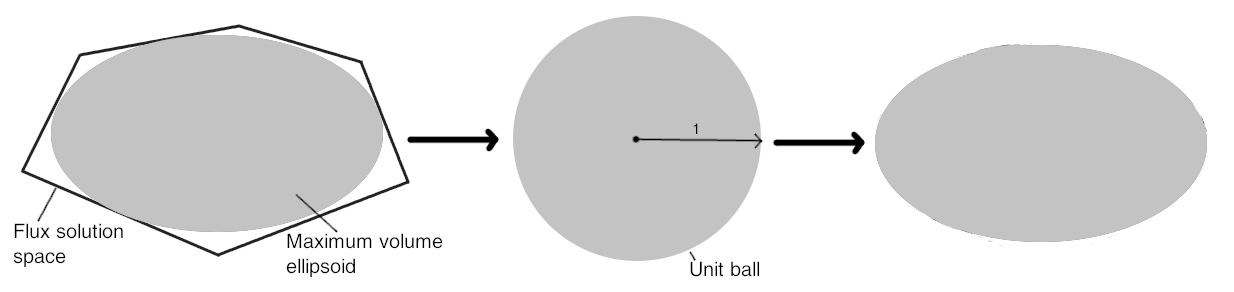
\includegraphics[scale=1.2]{fig2.png}
	\caption{\textbf{Rounding and transformation of the solution space by the CHRR algorithm}
The flux solution space is an irregular polytope and is rounded to an ellipsoid by using a maximum volume inscribed ellipsoid function. Next, the ellipsoid is transformed to a unit ball, where coordinate hit-and-run sampling takes place. Finally, the transform is reversed to give the original sample points. Adapted from Haraldsdottir \textit{et al}. (2017) supplementary methods\cite{Haraldsdottir}.
}
\label{figure:2}
\end{figure}

\pagebreak
\subsection*{Comparing the three sampling algorithms in meaningful biological contexts}
Our work evaluates the three modern samplers available in the COBRA software package: ACHR, OPTGP and CHRR. To the extent of our knowledge, these samplers have not been comprehensively compared to one another, making it unclear for users which sampler algorithm provides the best performance. Previous comparisons, such as those between the gpSampler {\&} OPTGP\cite{Megchelenbrink} and ACHR {\&} CHRR\cite{Haraldsdottir}, used limited measures of convergence and did not assess any differences in the flux probability distribution obtained. 

Here, we assess the performance of the algorithms against one another in four main areas; convergence to a stationary uniform sample, flux probability distributions produced, run time and ease of use. To achieve this, a variety of measures of convergence will be used to assess the required sample size to reach convergence at a wide range of network dimensions. Using this information, run time per sampling step on typical laptop and desktop machines will be recorded. The flux probability distributions produced by each sampler will be compared to investigate any differences in the samples produced from networks with a variety of properties. 

Finally, the best-performing sampler is assessed from an end-user standpoint in the context of a breast cancer cell and a plant leaf cell metabolic model.

% \begin{eqnarray}
% \label{eq:schemeP}
% 	\mathrm{P_Y} = \underbrace{H(Y_n) - H(Y_n|\mathbf{V}^{Y}_{n})}_{S_Y} + \underbrace{H(Y_n|\mathbf{V}^{Y}_{n})- H(Y_n|\mathbf{V}^{X,Y}_{n})}_{T_{X\rightarrow Y}},
% \end{eqnarray}

\section*{Materials and methods}
\subsection*{COBRA Toolbox and COBRApy setup}
COBRA Toolbox version 2.0.0 and COBRApy version 0.13.0 were installed. The linear programming solver used was Gurobi version 8.0.0 and the Toolbox was run on MATLAB version R2018a. 

The samplers were used in accordance with COBRA documentation\cite{docUniform}. For the CHRR sampler, the sampling density (nStepsPerPoint) was set to $8 \cdot dimensions^{2}$. When doing convergence comparisons, the optimal percentage parameter (optPercentage) was set to 0 to ensure that FBA analysis returned all potential solutions.

The ACHR sampler Python and MATLAB versions were compared. The MATLAB version of ACHR had a very slow run time per step, whereas the COBRApy version was around 20 times faster per step. The flux distributions produced by the two versions were compared at high step counts and negligible differences between the two samplers were found. Therefore going forward, the Python version was chosen to be compared to the other two samplers. 

\subsection*{Models}
To compare the performance of the samplers, four metabolic models with a varying number of reactions and metabolites were obtained in COBRA model format \textbf{(Table \ref{table:2})}. A small toy model was created using the the COBRA Toolbox function \texttt{createModel}. 

\begin{table}[!ht]
\begin{adjustwidth}{-2.25in}{0in}
\centering
\caption{
 {\bf Models used in the investigation.}}
\begin{tabular}{|>{\raggedright}p{3cm}>{\raggedright\arraybackslash}p{1.75cm}>{\raggedright\arraybackslash}p{1.5cm}>{\raggedright\arraybackslash}p{1.85cm}>{\raggedright\arraybackslash}p{2.75cm}>{\raggedright\arraybackslash}p{6cm}|}
\hline
\textbf{Model name} & \textbf{Metabolites} & \textbf{Reactions} & \textbf{Dimensions*} & \textbf{Average degree} & \textbf{Biological relevance} \\
\hline \hline
\textbf{Small toy} & 5 & 6 & 3 & 1.2 & NA \\
\hline
\textbf{\textit{E. coli }core (1)} & 72 & 95 & 24 & 1.32 & \textit{Escherichia coli} core metabolism \\
\hline
\textbf{\textit{T. maritima} (2)} & 570 & 652 & 57 & 1.14 & Central metabolic network of thermophilic bacteria \textit{Thermotoga maritima} \\
\hline
\textbf{Human RBC (3)} & 342 & 469 & 130 & 1.37 & Human erythrocyte (red blood cell) \\
\hline
\end{tabular}
\begin{flushleft} Source: 1) http://bigg.ucsd.edu/models/e\_coli\_core, 2)  http://bigg.ucsd.edu/models/iLJ478, 3) http://bigg.ucsd.edu/models/iAB\_RBC\_283
\\$*$ Number of dimensions in the solution space polytope. This corresponds to the number of non-zero flux reactions in the model and is therefore a better measure of network complexity than number of reactions.
\end{flushleft}
\label{table:2}
\end{adjustwidth}
\end{table}

\subsection*{Assessing convergence}
To estimate which sampler reached convergence in the fewest sampling steps and run time, a variety of methods to detect non-convergence were employed.

All four models were run on each of the three samplers for 20,000 sampling steps. This was repeated three times for each model to produce three sampling chains. In all cases, the flux probability distribution analysed was the objective reaction. In the small toy model, the reaction which totalled the output of the network was set to the objective. In the three BiGG models (\textit{E coli} core, \textit{T. maritima} and human RBC) the objective was set to the biomass reaction.

\subsubsection*{Running mean plots}
The mean of the flux probability distribution for the objective function was calculated at sample sizes of 100 to 20,000, in steps of 100 samples. The three sampling chains were plotted on the same axis for visualisation.

\subsubsection*{Gelman-Rubin}
The Gelman-Rubin diagnostic test compares within-chain variance with between-chain variance. The Gelman-Rubin diagnostic doesn’t look for convergence, instead it estimates the factor the variance between and within chains will decrease by, when the number of samples (n) tends towards infinity\cite{Sinharay}.
The resulting value is the potential scale reduction factor (PSRF)\textbf{(Equation 1)}. If the PSRF is close to 1, then there is likely to be no reduction in variance between the current sample and a sample size approaching infinity. Therefore, the closer the PSRF is to 1, the less evidence of non-convergence and increased likelihood that the sample is close to a uniform stationary distribution\cite{Brooks}.

\begin{eqnarray}
\label{eq:test}
PSRF = \sqrt{\frac{n-1}{n} + \frac{1}{n} \cdot \frac{B}{W}}
%  \caption{\textbf{Equation 1:} Where $B$ is the variance between the mean of the chains and $W$ is the variance within the mean of the chains. $N$ is the number of samples within the chain\cite{Sinharay}.}
\end{eqnarray}

The Gelman-Rubin PSRF value was calculated from three chains at sample sizes of 100 to 20,000, in steps of 100 samples. The first sampled value of each chain were compared to ensure that the chains started from varying areas of the flux distribution to comply with assumptions for the Gelman-Rubin diagnostic\cite{Brooks}. The \texttt{psrf} function from the MCMC Diagnostics Toolbox for MATLAB was used to calculate the PSRF\cite{mcmcdiag}.

\subsubsection*{XY deviation}
The method of calculating XY deviation was adapted from Megchelenbrink \textit{et al.} (2014)\cite{Megchelenbrink}. The mean flux value was normalized using the minimum and maximum flux value for the reaction \textbf{(Equation 2)}. The difference the mean flux of each chain at a range of sample sizes was compared to that of the mean flux of three chains of 20,000 samples. The larger the difference between the two samples, the larger the difference between the distributions of the two samples and therefore evidence for non-convergence. 

\begin{eqnarray}
\label{eq:test2}
XY deviation = \sqrt{(X-Y)^{2}}
%  \caption{\textbf{Equation 2:} Where $X$ is the mean of chain at a sample size $<$20,000, Where $Y$ is the mean of 3 chains of 20,000 samples, representing the the mean flux of the stationary uniform sample. 
\end{eqnarray}

\subsubsection*{Flux histograms}
The flux probability distributions at a range of sample sizes were plotted on the same axis to allow for visual comparison of the distributions produced. 50 histogram bins were used for all sample sizes to allow for fair comparison of the smoothness of the probability distribution produced.

\subsubsection*{Raftery \& Lewis convergence diagnostic}
The Raftery \& Lewis convergence diagnostic estimates the run-length needed to reach a stationary sampling distribution. It uses an individual chain to make this estimate. The estimate is based on the two-state Markov chain theory and is made by calculating the run length needed to predict a certain quantile of the target distribution. The user must define the quantile of interest, the level of accuracy required and the desired probability of obtaining that level of accuracy. The \texttt{raftery.diag} function from the CODA package for R was used to calculate this diagnostic on a chain from each sampler with a length of 20,000\cite{Plummer}. The user-specified parameters used were: q=0.025, r=0.005, s=0.95. Where: q is the quantile to be estimated, r is the margin of error of the estimate, s is the probability of obtaining the estimate.

\subsection*{Run times}
Run times on MATLAB were tested using the tic and toc functions\cite{tictoc}. In Python, the run time was calculated using the time module\cite{time}. 1,000 sampling steps were run in order to produce an estimate of run time per sampling step. The four models \textbf{(Table \ref{table:2})} were run on each sampler on a laptop (7GiB RAM and a AMD A10-4655M processor, 4 cores and a maximum capacity of 2GHz) and desktop computer (Intel Xeon ES-1650V4 processor, 6 cores and a maximum capacity of 4GHz). 

\subsection*{Comparing flux distributions} 
To identify any differences, the flux distributions produced by the four samplers were compared using a range of methods. 

To compare reactions with different ranges of flux variability, the flux values were normalized to a -1 to 1 scale using the maximum and minimum flux values obtained for that reaction across all three samplers.

\subsubsection*{Probability distribution functions}
The estimated probability function for each flux distribution was produced using the MATLAB function \texttt{ksdensity}\cite{ksdensity}. The probability density function for each sampler was plotted on the same axes to look for differences between the samples by eye. This was repeated in all four models.

\subsubsection*{ANOVA}
A one-way analysis of variance (ANOVA) was carried out to assess if the samples produced by the three samplers all came from the same sampling distribution. The non-parametric Kruskal-Wallis test at a significance level of 0.95 was used. The objective reaction for each of the four models was used to make this comparison. For the small toy and \textit{E. coli} core model, this test was carried out below (n = 1000, where n is number of samples) and above (n = 20,000) convergence.

\subsubsection*{Difference in normalized means}
Sampled reaction flux values produced were normalized to a -1 to 1 scale. For each model, the normalized means of CHRR and OPTGP was compared to that of ACHR for every reaction in the model. The overall mean difference between the samplers for each model was then visualised as a bar chart. Zero-flux reactions were excluded from this analysis.

To further visualise the differences between the samplers, the normalized means of each reaction were plotted on a scatter chart with one sampler against another. The closer to x = y, the less difference between the means of the two samplers. This was repeated in all four models.

% Results and Discussion can be combined.
\section*{Results}

Convergence is reached when the sampling chain has fully explored all areas of the flux solution space and produces a stationary, uniform distribution. Therefore, to produce an accurate flux probability density for each reaction, samplers must be run beyond convergence. A range of techniques including plotting the running mean, the Gelman-Rubin diagnostic test, and XY deviation are used here to detect non-convergence between sampling chains. 

The running mean of each chain between 100 and 20,000 sampling steps is calculated and then plotted for each sampler. Before convergence, the means of each chain are very different from each other and as more samples are added to the chain, the mean varies dramatically. For the small toy model, the running means shows that the OPTGP sampler appears to reach convergence in the greatest number of samples \textbf{(Fig \ref{figure:3}A)}. At between 100 and 5,000 samples, the three OPTGP chains have the largest difference in means compared to ACHR and CHRR. For ACHR and CHRR, the chains become much more similar and there is little variation in the mean value as the number of samples approaches 10,000. For OPTGP, this levelling off occurs at around 15,000 samples, suggesting that convergence occurs later. 

\begin{figure}
\begin{adjustwidth}{-2.25in}{0in}
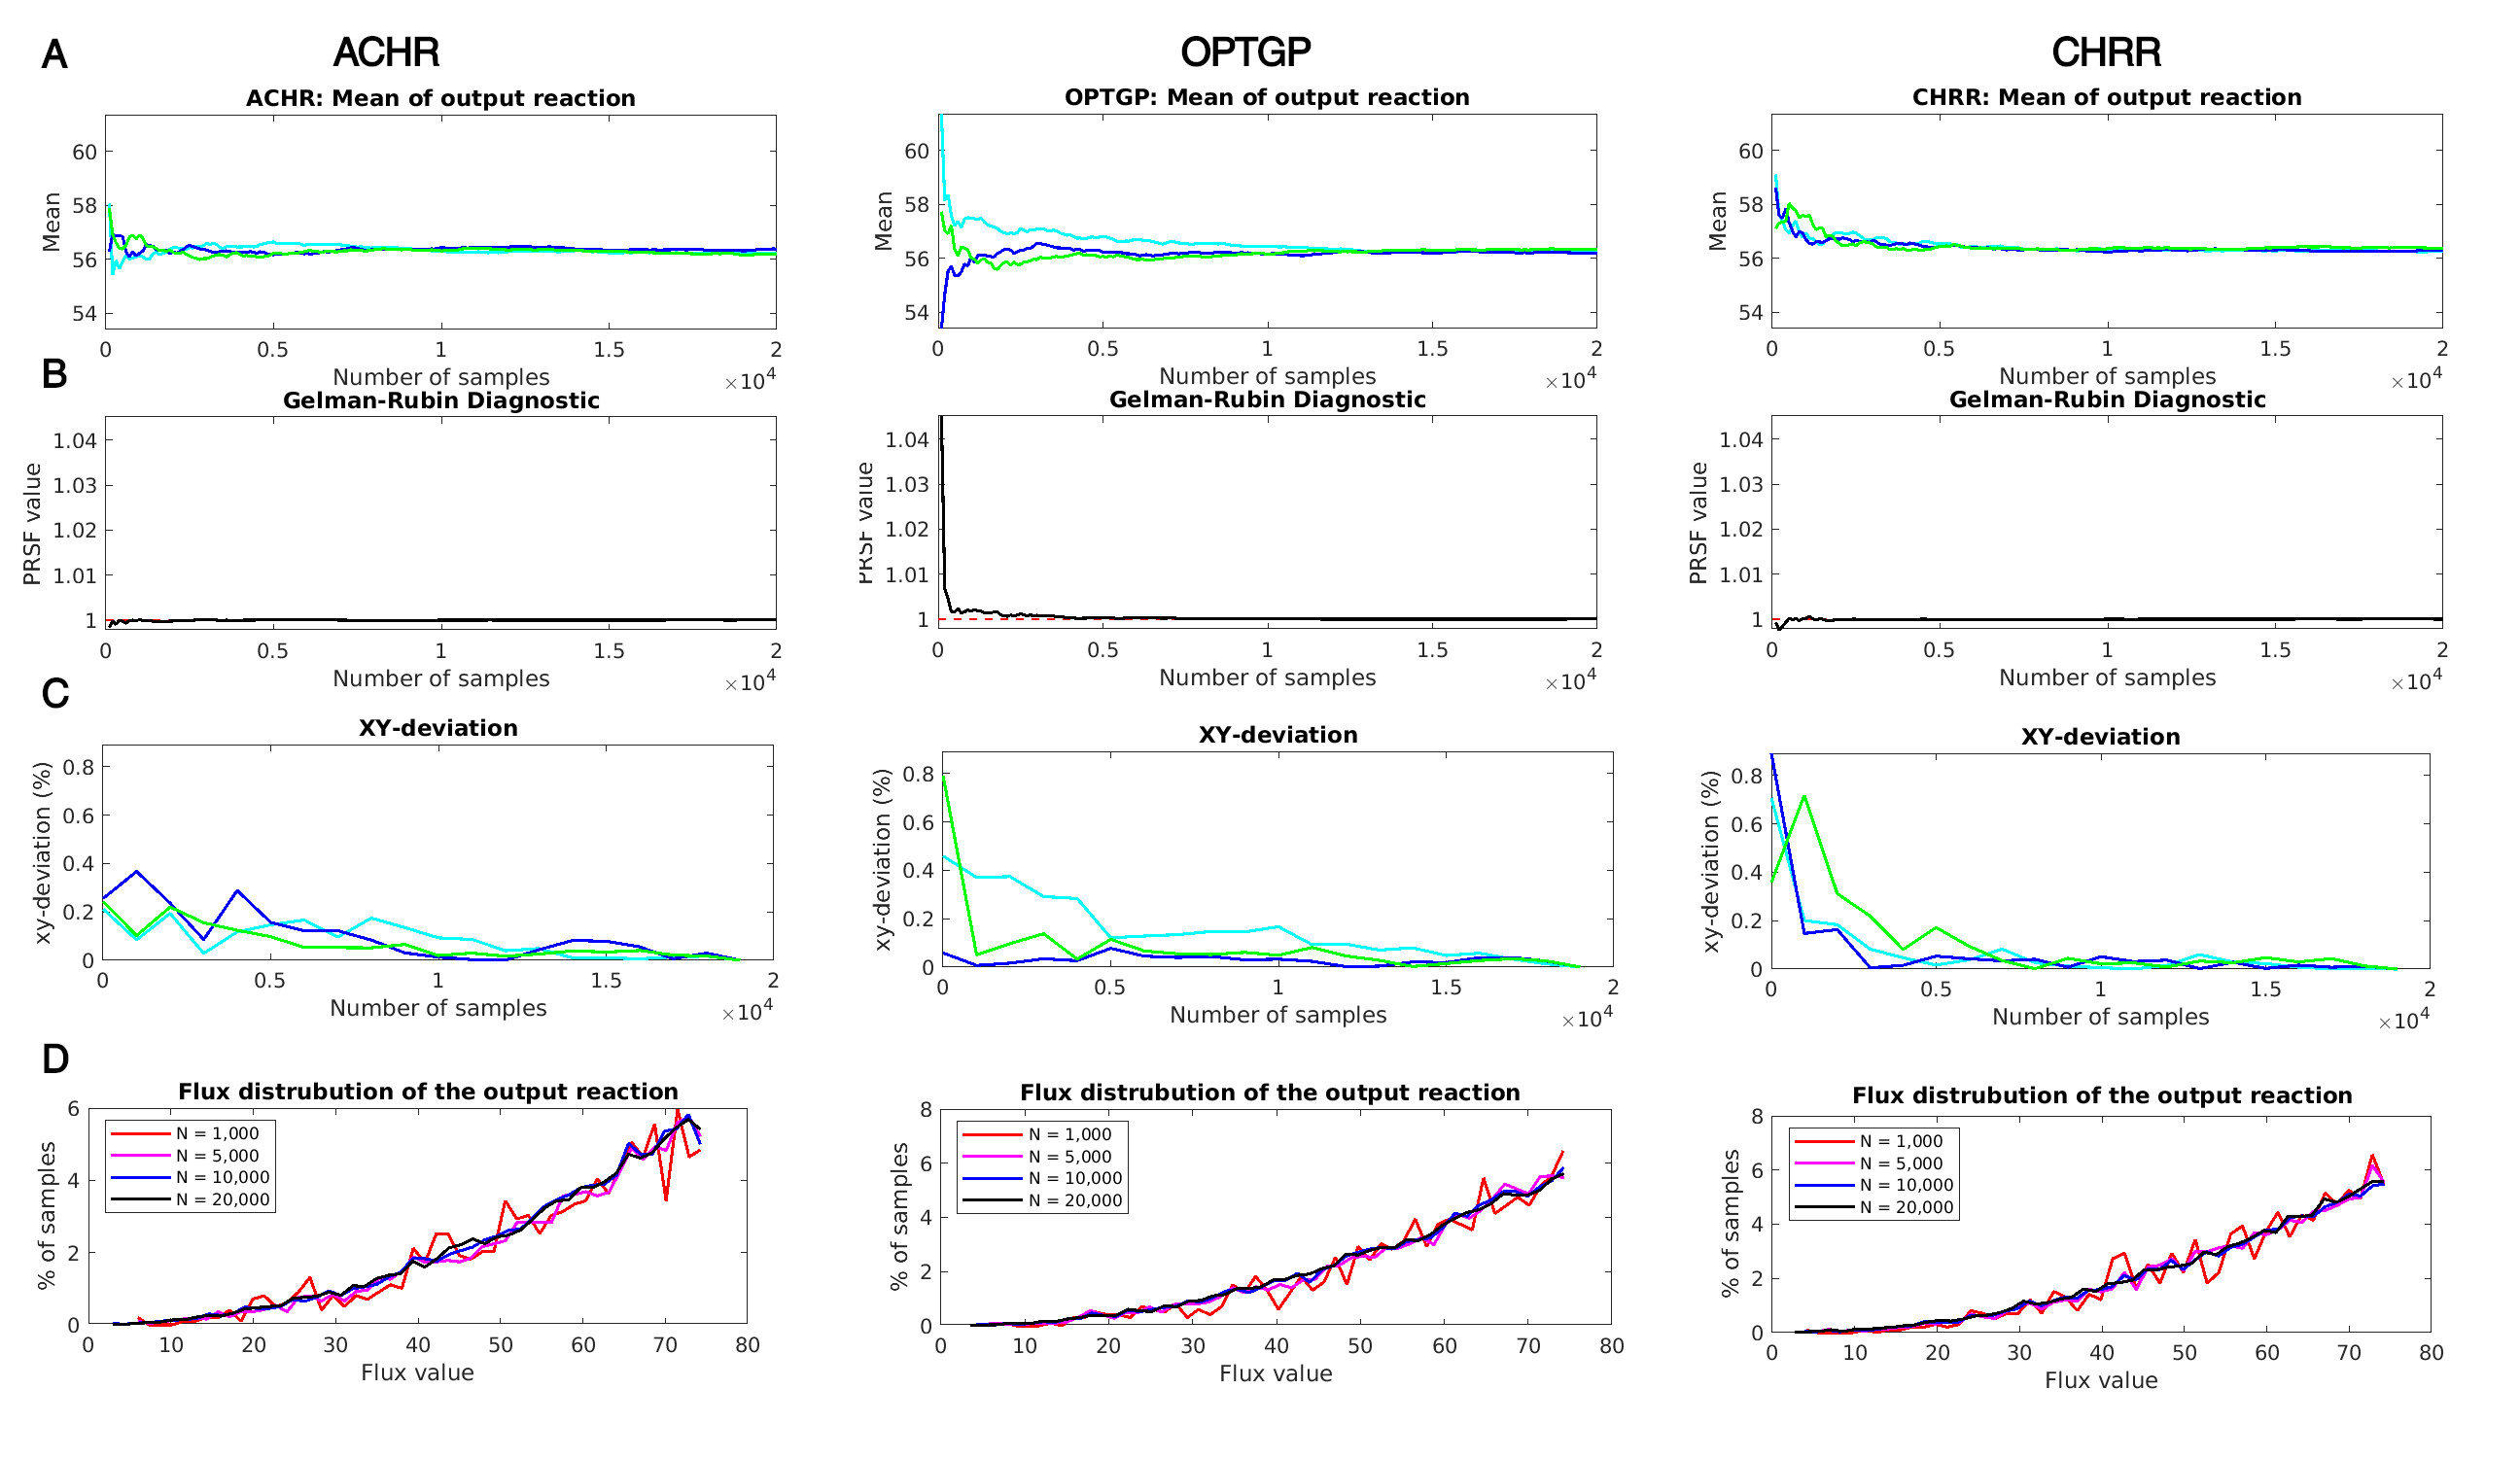
\includegraphics[scale=0.45]{fig3.png}
\caption{\textbf{Evidence of convergence for the small toy model}\\
A) Running mean of three chains. B) Gelman-Rubin PSRF value. C) XY deviation of the three chains. D) Flux histograms at four sample sizes. 
}
\label{figure:3}
\end{adjustwidth}
\end{figure}

These results are confirmed by the Gelman-Rubin PSRF value \textbf{(Fig \ref{figure:3}B)}. The ACHR and CHRR PSRF values reach 1 at around 1,000 iterations. A PSRF value close to 1.0 indicates that the sample produced is likely to be the same as that produced at a extremely high sample size. In comparison, the OPTGP PSRF value does not reach 1 until a chain length of around 4,000 samples. Both the running mean plots and the Gelman-Rubin PSRF value indicate that all three samplers reach convergence by 20,000 samples.

XY deviation is a measure of how much deviation there is between the mean at low sample sizes (100 to 19,900) compared to at a large sample size (20,000). The XY deviation of the three chains produced by each sampler show that the means of CHRR and OPTGP start furthest away from the mean at 20,000 samples \textbf{(Fig \ref{figure:3}C)}. By a sample size of 10,000, the three CHRR chains have the lowest amount of difference from the mean at 20,000 samples, suggesting that CHRR reaches convergence at the lowest sample size. Despite having initially low XY deviation, ACHR XY deviation for all three chains is greater than CHRR at 10,000 samples.

The flux distribution for one chain was plotted at four different sample sizes and visualised using a histogram (Fig \ref{figure:3}D). The same bin size was used at all five sample sizes to allow for a comparison of the smoothness of the distributions. The distributions for all three samplers become smooth at around 10,000 iterations. For all three samples, there is very little difference in the overall shape of the distributions between a sample size of 1,000 and 20,000. This suggests that even at a low sample size of 1,000 iterations, the samplers have explored the flux solution space to a level sufficient for a good estimation of the probability density.

For the small toy model, ACHR and CHRR appear to converge at the lowest sample sizes, and OPTGP convergence appears to be at a higher sample size. This is an unexpected result as previous literature suggested that OPTGP is an improvement on the gpSampler, an algorithm which is closely related to ACHR\cite{Megchelenbrink}.

To investigate if the samplers reached convergence at different points for flux solution spaces with higher dimensions, the convergence assessment was carried out in the same way on the \textit{E. coli} core, \textit{T. maritima} and human RBC models \textbf{(Table \ref{table:4})}. 

\begin{table}[!ht]
\begin{adjustwidth}{-1.4in}{0in}
\centering
\caption{Results from three methods of assessing convergence of the samplers.}
\begin{tabular}{|>{\raggedright}p{4cm}|>{\raggedright\arraybackslash}p{2cm}|>{\raggedright\arraybackslash}p{3cm}>{\raggedright\arraybackslash}p{3cm}>{\raggedright\arraybackslash}p{3cm}|}
\hline
\textbf{Model (dimensions)} & \textbf{Sampler} & \multicolumn{3}{c|}{\textbf{Method of detecting non-convergence}} \\ \cline{3-5} 
 &  & \textbf{Running means, Gelman Rubin diagnostic test, and XY deviation} & \textbf{Flux probability distribution} & \textbf{Raftery \& Lewis convergence diagnostic} \\ \hline
\textbf{Small toy (3)} & ACHR & 5,000 & \textgreater{}1,000 & 3,725 \\ \cline{2-5} 
 & OPTGP & 10,000 & \textgreater{}1,000 & 3,771 \\ \cline{2-5} 
 & CHRR & 6,000 & \textgreater{}1,000 & 3,710 \\ \hline
\textbf{\textit{E. coli }core (24)} & ACHR & \textgreater{}20,000 & \textgreater{}20,000 & 4,654 \\ \cline{2-5} 
 & OPTGP & \textgreater{}20,000 & 10,000-20,000 & 4,539 \\ \cline{2-5} 
 & CHRR & 7500 & 5,000-10,000 & 3,710 \\ \hline
\textbf{\textit{T. maritima} (57)} & ACHR & \textgreater{}20,000 & \textgreater{}20,000 & 134,215 \\ \cline{2-5} 
 & OPTGP & 10,000 & \textgreater{}20,000 & 8,706 \\ \cline{2-5} 
 & CHRR & 4000 & 5,000-10,000 & 3635 \\ \hline
\textbf{Human RBC (130)} & ACHR & \textgreater{}20,000 & \textgreater{}20,000 & 205,590 \\ \cline{2-5} 
 & OPTGP & \textgreater{}20,000 & \textgreater{}20,000 & 24,688 \\ \cline{2-5} 
 & CHRR & 4000 & 5,000-10,000 & 3,771 \\ \hline
\end{tabular}
\label{table:4}
\end{adjustwidth}
\end{table}

\begin{figure}[!ht]
\begin{adjustwidth}{-2.25in}{0in}
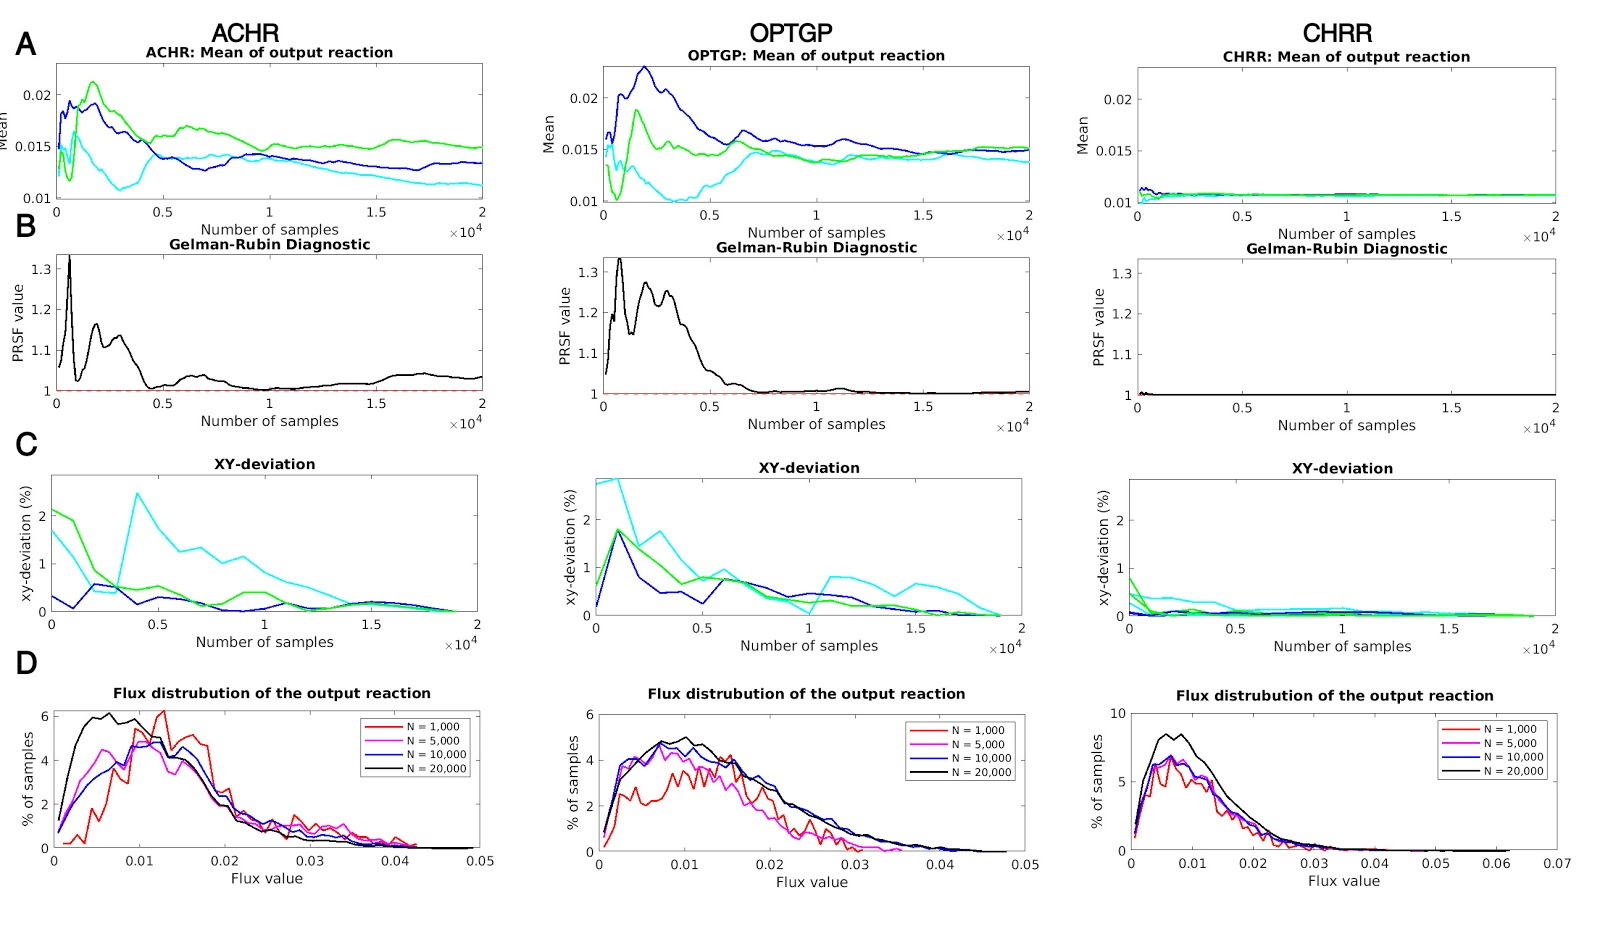
\includegraphics[scale=0.34]{Fig4.png}
\caption{{\bf Evidence of convergence for the human RBC model.}
The flux solution space of the model is in 130 dimensions. A) Running mean of three chains. B) Gelman-Rubin PSRF value. C) XY deviation of the three chains. D) Flux histograms at four sample sizes.}
\label{figure:4}
\end{adjustwidth}
\end{figure}

It was found that for the OPTGP and ACHR samplers, as the dimensionality of the solution space increases, the number of sampling steps needed to reach convergence also increases. In the human RBC model (dimensions = 130), convergence for the ACHR and OPTGP sampler is estimated to be above 20,000 iterations \textbf{(Fig \ref{figure:4})}. The running means show that for the ACHR and OTPGP samplers, at 20,000 iterations, there are still large differences between the means of each chain \textbf{(Fig \ref{figure:4}A)}. This is reflected in the high PSRF values for ACHR and OPTGP \textbf{(Fig \ref{figure:4}B)}. In comparison, CHRR appears to reach convergence very quickly, by around 5,000 iterations. The flux distributions for a single chain of the ACHR sampler vary in shape between the four sample sizes, with the distribution of the sample size at 1,000 being very different from that at 20,000 \textbf{(Fig \ref{figure:4}D)}. This indicates that at 1,000 iterations, the ACHR sampler hasn’t fully explored the flux solution space for the human RBC model. 

The Raftery \& Lewis test uses an individual sampling chain to give an estimate of the number of sampling steps needed to reach a stationary sampling distribution. The results of the Raftery \& Lewis test show that for ACHR and OPTGP, as the dimension of the flux solution space increases, the number of samples to convergence increases dramatically \textbf{(Table \ref{table:4})}. However, the CHRR sample size remains fairly constant at around 3,700 samples. This results reflects the conclusions drawn from the multiple chain methods (running means, Gelman-Rubin and XY deviation) for \textit{T. maritima} and human RBC model. The \textit{E. coli} core model appears to have a higher convergence for the CHRR sampler using these multiple chain methods, which highlights the importance of using a varied range of methods to assess convergence. 

In summary, these results suggest that CHRR is the best performing sampler because the number of samples to convergence appears to remain fairly constant as the dimensionality of the flux solution space increases. However, findings presented in Haraldsdottir \textit{et al.} (2017) suggest that when the dimension increases above 1,000, the number of sampling steps to convergence increases dramatically\cite{Haraldsdottir}. In comparison, ACHR and OPTGP sampling steps to convergence seems to increase as the dimensionality of the flux solution space increases. Raftery \& Lewis convergence diagnostic results suggest that OPTGP performs better than ACHR, but this wasn’t shown by other methods of assessing convergence. 

\subsection*{OPTGP has the fastest run time per sampling step}
The run time of the algorithm per sampling step is an important consideration. Computational biologists using FBA often need to run many repeats of sampling on highly dimensional models under different constraints which simulate \textit{in silico} gene knockouts, enzyme inhibition or limiting environmental factors. 

The run time was assessed by running the four models on each sampler for 1,000 steps on both a laptop and desktop computer \textbf{(Fig \ref{figure:5})}. In general, the run time per step increased as the dimension of the flux solution space increased. Interestingly, for the OPTGP and ACHR samplers, the \textit{T. maritima} model (57 dimensions) took longer per step than the human RBC model (130 dimensions). This could be because the \textit{T. maritima} model contained more metabolites and reactions than the human RBC model \textbf{(Methods Table \ref{table:2})}. Unlike the CHRR algorithm, the ACHR and OPTGP algorithms do not remove the zero-flux reactions in the warm-up phase, so the output of these reactions is calculated in each sampling step. OPTGP was the fastest per sampling step for networks of greater than 24 dimensions (\textit{E. coli} core). ACHR had very similar run time per sampling step as OPTGP. CHRR was up to 27.5 times slower than OPTGP per sampling step. The human RBC model (130 dimensions) took around 3s per sampling step on the desktop computer. This difference could be because CHRR is implemented using MATLAB.


\begin{figure}[!h]
\centering
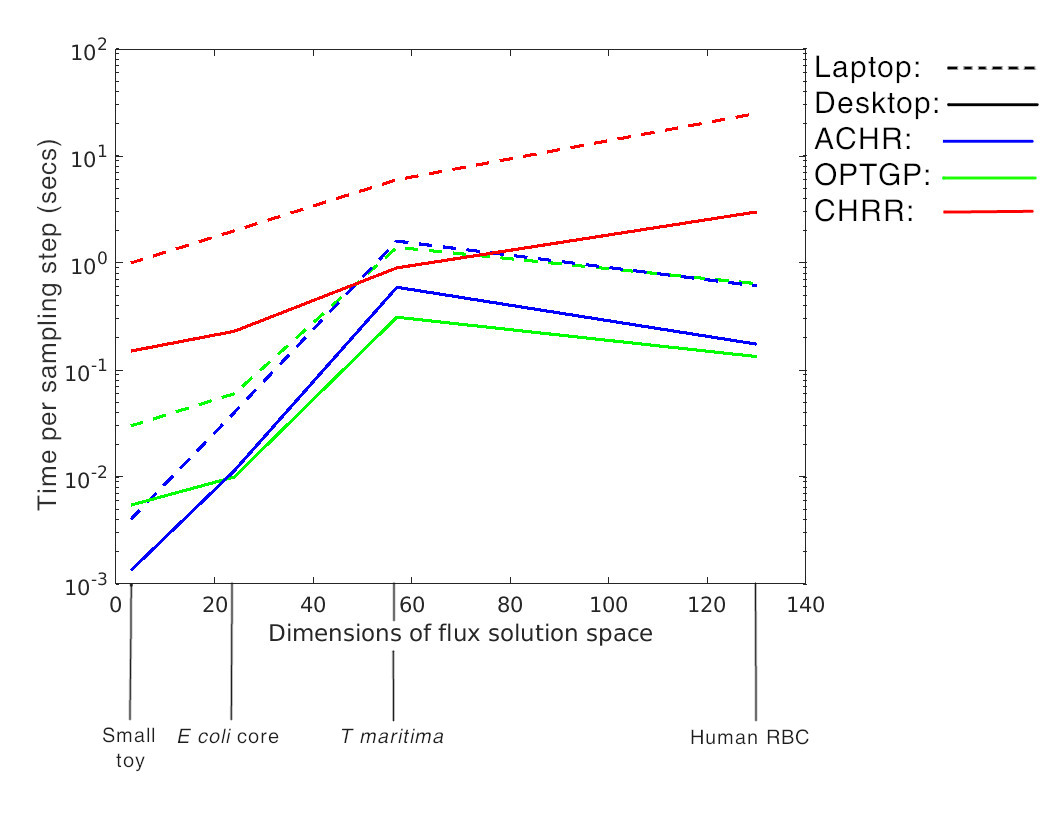
\includegraphics[scale=0.6]{fig5.png}
\caption{\textbf{Run times of the four models on each sampler.}\\
Run time on both a laptop and desktop computer were compared.
}
\label{figure:5}
\end{figure}

\subsection*{The three samplers produced similar flux distributions}
The sampled flux values for each reaction of the four models were plotted as probability density functions and compared by eye. Although there was some small differences in the plots, neither one of the samplers consistently produced different results. 

A one-way analysis of variance (ANOVA) was used to investigate if the samples produced by each sampler were likely to have come from the same distribution \textbf{(Table \ref{table:5})}. Values less than 0.05 suggest that there is a significant difference between the flux distributions produced by the three samplers. At 1,000 sampling steps, only the samples from the small toy model appeared to be from the same sampling distribution. For the three larger models, the test concluded that the samples were drawn from different distributions. However, at 20,000 samples, all four models were shown to be drawn from the same sampling distribution. This suggests that there is little difference between the sampling distributions produced by the three samplers. The differences between the three samplers at 1,000 samples might be due to the very low number of samples, meaning the samplers haven’t fully explored the flux distribution space in the higher dimension models. 

\begin{table}[!ht]
%\begin{adjustwidth}{-1.25in}{0in}
\centering
\begin{tabular}{|>{\raggedright}p{4cm}>{\raggedright\arraybackslash}p{4cm}>{\raggedright\arraybackslash}p{4cm}|}
\hline
\textbf{Model} & \textbf{At 1,000 samples} & \textbf{At 20,000 samples} \\ \hline \hline
\textbf{Small toy} & 0.8314 & 0.9588$*$ \\ \hline
\textit{\textbf{E. coli core}} & \textless{}0.05 & 0.8340$*$ \\ \hline
\textit{\textbf{T. maritima}} & \textless{}0.05 & 1 \\ \hline
\textbf{Human RBC} & \textless{}0.05 & 0.1287 \\ \hline
\end{tabular}
\caption{\textbf{ANOVA test to compare the flux distributions of the objective reaction from 3 samplers.} \\ $\alpha = 0.05$ (95$\%$ confidence). 
\\ $*$ Above estimated convergence for all 3 samplers.}
\label{table:5}
%\end{adjustwidth}
\end{table}

To look for consistent differences between the samplers, the means of the normalized flux value for each reaction was compared. The total difference between each sampler for all reactions in the model was then averaged to give a final normalized difference score \textbf{(Fig \ref{figure:6})}. The results show that on average, ACHR and CHRR produced more similar results than OPTGP. In all four models, CHRR produced a higher mean flux than ACHR. OPTGP varied the most from the other two samplers. There appeared to be no association between flux solution space dimensionality and the difference between samplers. Overall, all three samplers produced very similar flux distributions.

\begin{figure}[!h]
\centering
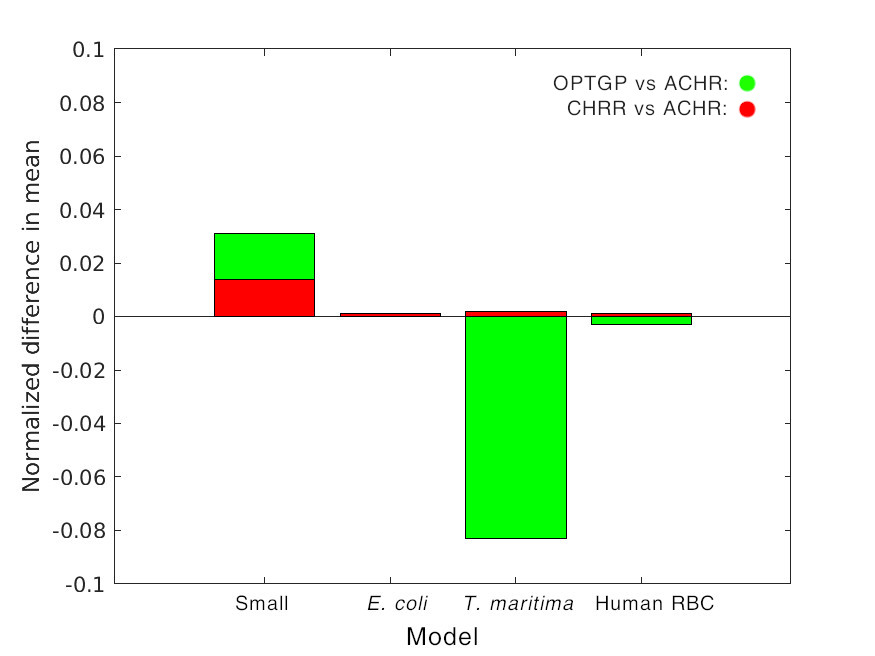
\includegraphics[scale=0.75]{fig6.png}
\caption{\textbf{Normalized differences in means between ACHR, OPTGP and CHRR for the four models.}\\
The normalized mean of each reaction in the four models was calculated. The average difference in the means for each model between the three samplers is shown. Green bars show the difference between OPTGP and ACHR, and red bars the difference between CHRR and ACHR. There was \textless{}0.001 difference between OPTGP and ACHR in the \textit{E coli} core model.
}
\label{figure:6}
\end{figure}

\pagebreak 
The differences between individual reactions from each of the models was investigated by plotting the normalized mean from one sampler against another \textbf{(Fig \ref{figure:7})}. The scatter plots for the \textit{T. maritima} model \textbf{(Fig \ref{figure:7}A)} and human RBC model \textbf{(Fig \ref{figure:7}B)} show that for some reactions, there is a larger difference between the means produced by the samplers. There is a larger difference between the three samplers for reactions which have a high and low normalized mean flux, but little difference for those with a normalized mean flux around zero. Examples of reactions from the \textit{T. maritima} model with high, low and close to zero mean flux are shown in \textbf{Figure \ref{figure:7}C}.

When comparing ACHR to OPTGP for both models, there is an equal amount of points above and below the x=y line, indicating that on average, neither sampler produced a mean flux higher than the other. However, when comparing ACHR to CHRR in both models, the majority of reactions with a positive flux mean lie above the x=y line, indicating that for these reactions, CHRR generally produces a higher mean flux value than ACHR. For reactions with a negative mean flux, the majority of points below the x=y line, indicating CHRR generally produces a lower mean flux value than ACHR for these reactions. This is also the case when comparing CHRR to OPTGP. These results indicate that perhaps CHRR oversamples the extreme flux values closer to the reaction constraints than OPTPG and ACHR, skewing the flux distribution towards more extreme values. 

\begin{figure}[!ht]
%\begin{adjustwidth}{-1.8in}{0in}
\centering
	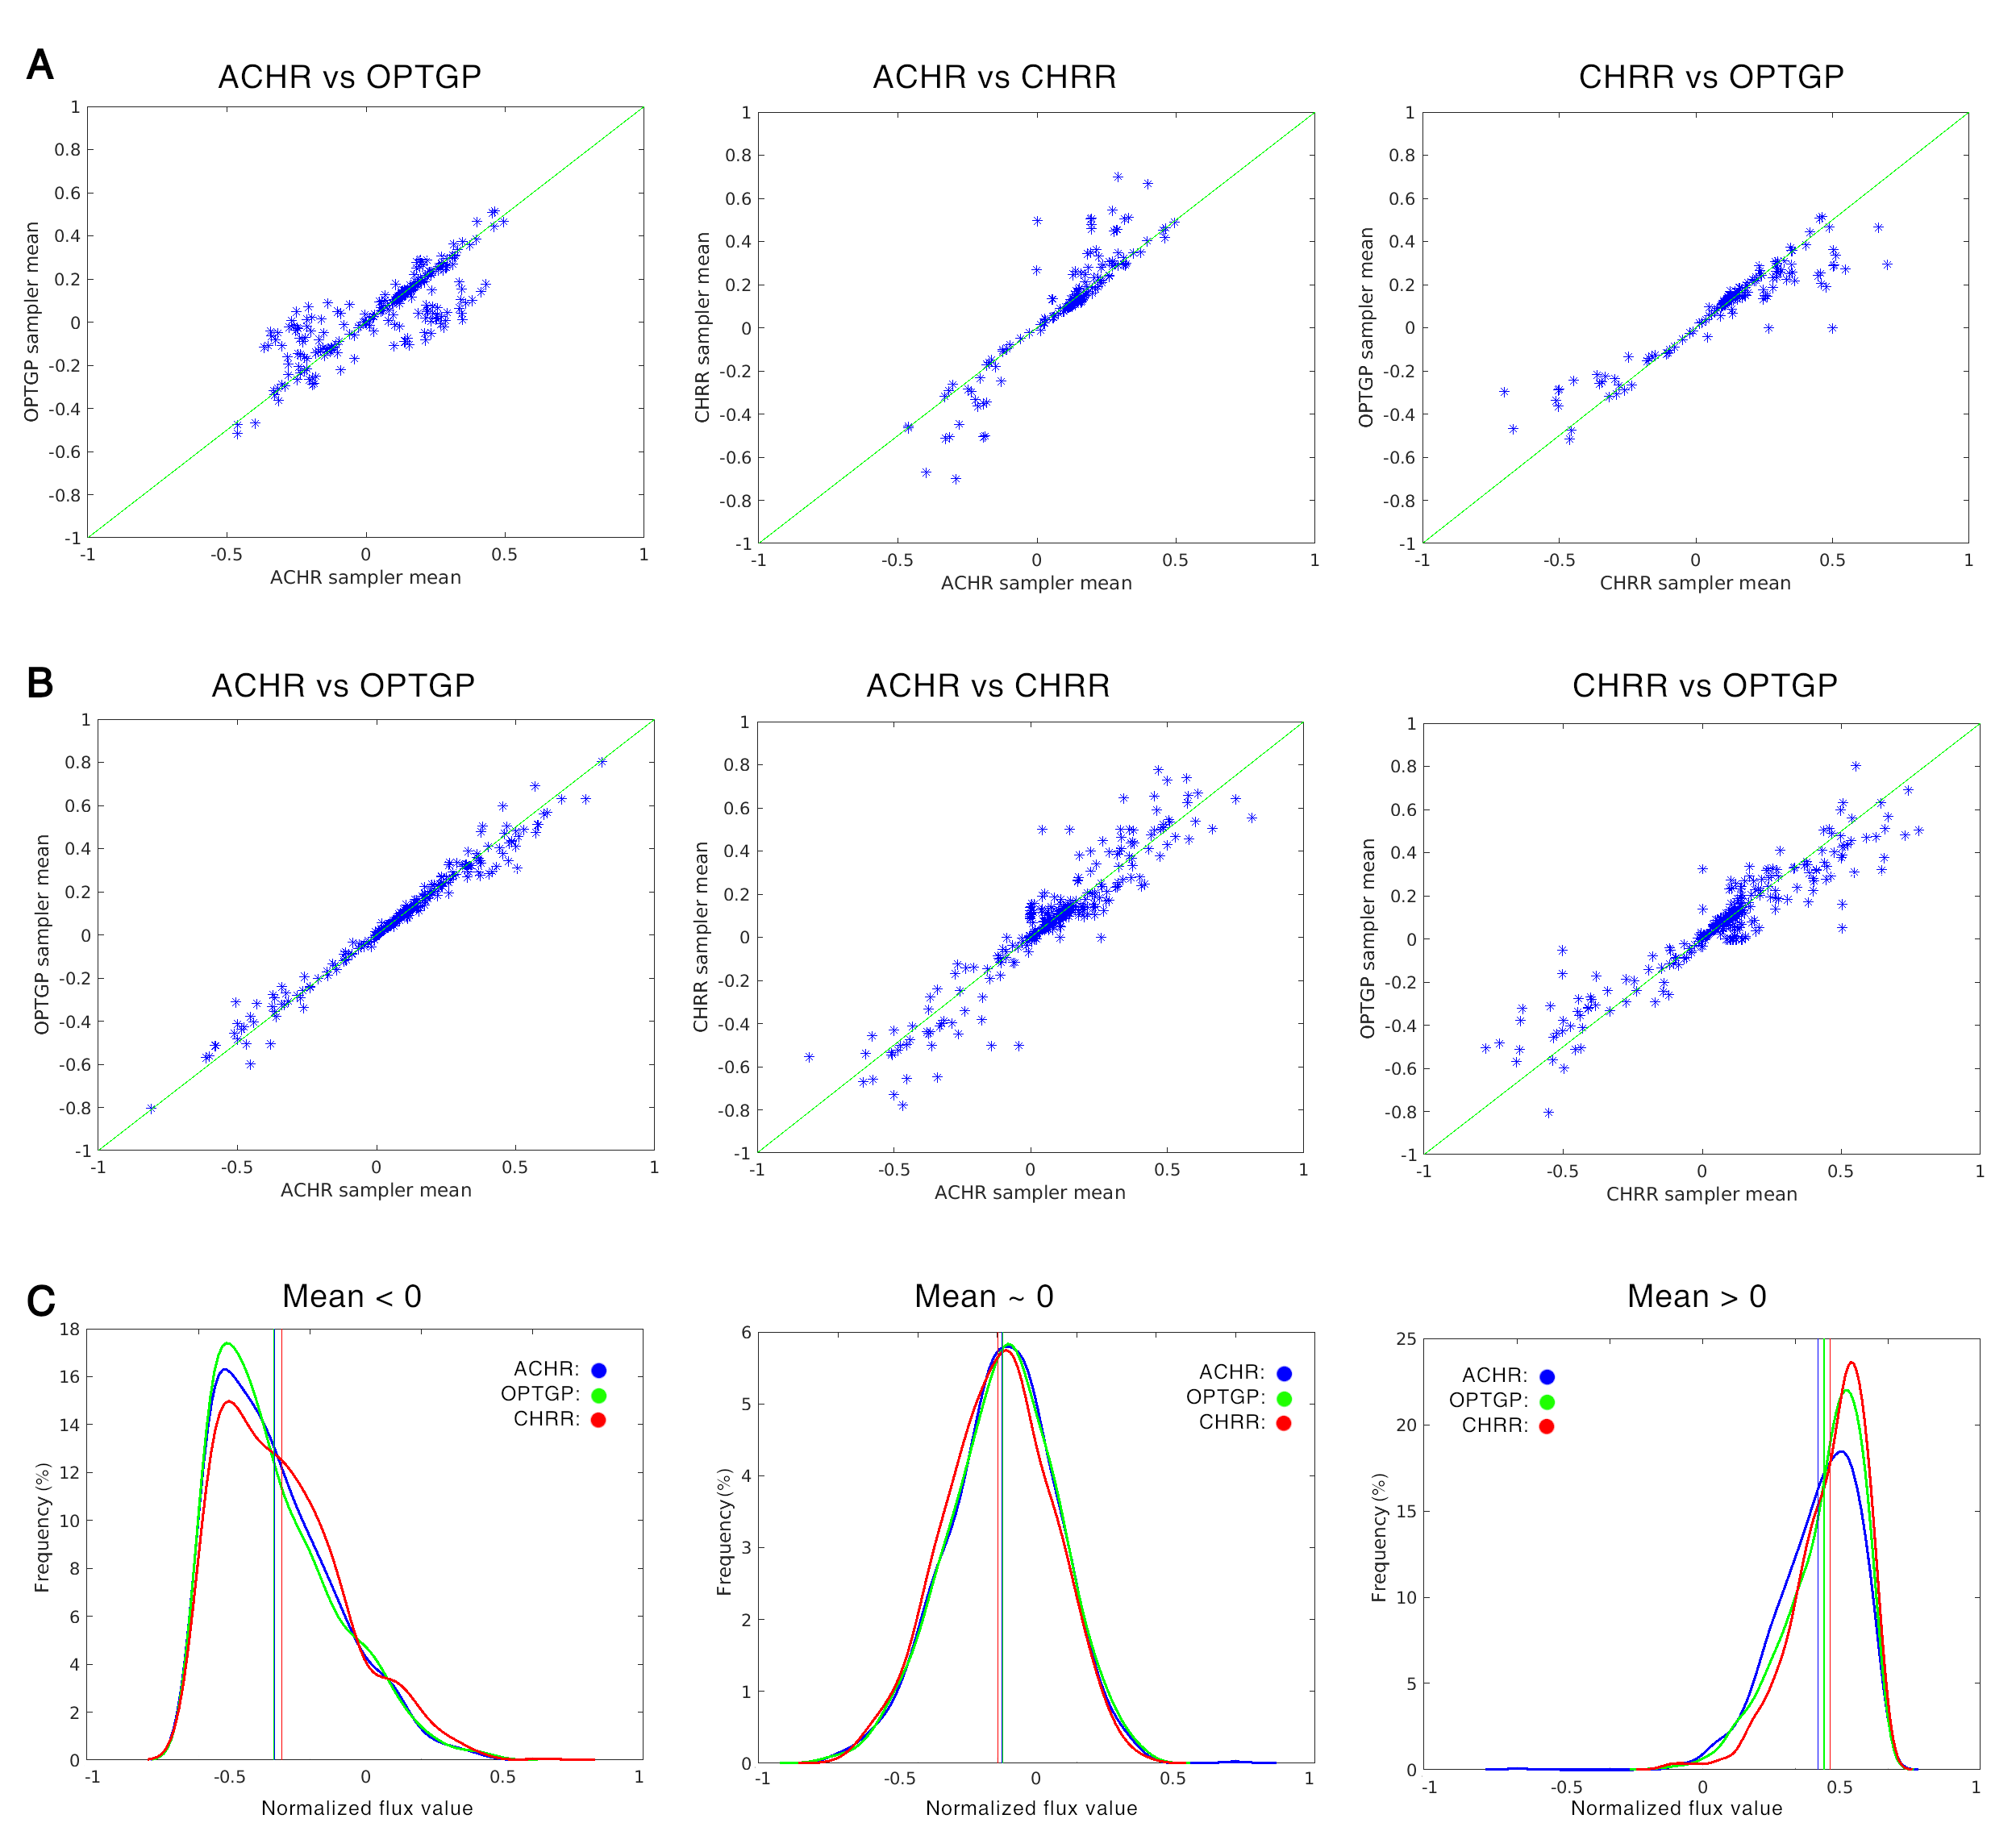
\includegraphics[scale=0.32]{fig7.png}
	\caption{\textbf{Investigating the difference between mean flux in individual reactions.}\\
A) Scatter plots comparing the normalized mean flux between samplers from reactions from the \textit{T. maritima} model. Number of samples = 20,000. \\ B) Scatter plots comparing the normalized mean flux between samplers from reactions from the human RBC model.  Number of samples = 20,000. \\ C) Flux probability distributions produced by the three samplers from three reactions from the \textit{T. maritima} model, with normalized means below zero, close to zero and above zero. Number of samples = 1,000 to highlight the differences between the samplers.
}
\label{figure:7}
%\end{adjustwidth}
\end{figure}

Overall, comparisons of the three samplers show that CHRR has a much lower number of sampling steps to convergence than OPTGP and ACHR, especially for highly dimensional flux solution spaces. The number of sampling steps to convergence for OPTGP and ACHR increases dramatically as the dimensionality of the flux solution space increases, whereas CHRR is less affected by this. This would indicate that CHRR is a better choice of sampler, especially for large and complex models such as genome-scale metabolic reconstructions, as the sampling chain doesn’t need to be run for as many steps as OPTGP and ACHR to reach convergence. OPTGP showed slightly better convergence than ACHR.

However, the run time of CHRR, implemented using MATLAB, is much greater than OPTPG and ACHR, which are implemented using Python. For the human RBC model, the most highly dimensional model tested (dimensions = 130), OPTGP and ACHR were around 30 times faster than CHRR. Therefore, it could be more efficient to run sampling chains for longer on the faster OPTGP and ACHR samplers. 

There did not appear to be any large differences between the flux distributions produced by the three samplers. Comparison of the mean flux distribution showed that in high dimension models, CHRR samples the flux distribution more readily near the maximum and minimum flux values. Network properties showed little correlation with differences between samplers, suggesting they are not affected differently by the network properties tested.

\subsection*{Application of uniform sampling to study a genome-scale metabolic networks - Lessons from breast cell models}
\label{cancer}
% Need to re-write this section so that biomass production is near-optimal to optimal (80% or higher) 
% Doing so will likely change the model dimension.... 
% This will change the numbers for run-time but hopefully not by much

\subsubsection*{The Warburg effect and the role of lactate dehydrogenase}
Under aerobic conditions, normally differentiated cells rely on oxidative phosphorylation to produce adenosine triphosphate (ATP) and provide energy for cellular processes. Cancer cells are distinct in that they rely on glycolysis, a less efficient process which is usually only used by to produce ATP under anaerobic conditions. This phenomenon, also known as the Warburg effect or aerobic glycolysis, is thought to be advantageous to proliferating cancer cells as it increases production of macromolecules which contribute to biomass, such as lipids, amino acids and nucleotides\cite{Heiden}.

Pyruvate is the metabolite at the junction of glycolysis and oxidative phosphorylation. In normal differentiated cells when oxygen is present, most pyruvate is decarboxylated to produce acetyl coenzyme A (acetyl-CoA), which enters the mitochondrial tricarboxylic acid (TCA) cycle and drives ATP production\cite{Heiden}. In proliferating tissue or under anaerobic conditions, pyruvate is converted to lactate by lactate dehydrogenase. Lactate dehydrogenase A (LDHA), the monomer which preferentially catalyses the reduction of pyruvate to lactate, has been identified as a potential therapeutic target and is a promising therapeutic for drug resistant cancers such as triple negative breast cancer\cite{Allison}\cite{Mack}. Both \textit{in vitro} and \textit{in vivo}, inhibition of LDHA using interfering RNA or small molecule inhibitors has been shown to induce cancer cell apoptosis, decrease tumorigenesis and cause regression of tumors\cite{Allison}\cite{Xie}.

To simulate the effects of inhibiting LDHA activity on breast cancer metabolism, a genome-scale metabolic reconstruction of breast cancer was analysed using flux sampling. Varying the constraints of the system allows \textit{in silico} inhibition of LDHA and comparison of flux probability distributions could give insights into the metabolic pathways that are likely impacted.  

\subsubsection*{Using the OPTGP sampler to generate flux distributions of breast cell metabolism}
Two genome-scale metabolic reconstructions, ‘iBreastCancer1771’ and ‘Breast Glandular cells’ were obtained from the Human Metabolic Atlas as COBRA models\cite{metatlas}\cite{Gatto}. These reconstructions were created using the INIT (Integrative Network Inference for Tissues\cite{Argen}) algorithm combined with data from RNAseq profiles for breast tumor cells and adjacent normal breast cells\cite{Gatto}. In the breast cancer model, an objective cancer biomass exchange reaction was included to assess the estimated cell growth and proliferation. The breast cancer model is made up of 5458 metabolites, 4300 reactions and can be reduced to 755 dimensions. The healthy cell model has 5969 metabolites, 5162 reactions and 1258 dimensions.

Haraldsdottir \textit{et al.} (2017) present results which show that for the CHRR sampler, the number of sampling steps to convergence is stays fairly constant as model dimension increases to up to 1,000\cite{Haraldsdottir}. Therefore it can be estimated that for the CHRR sampler, the number of steps to convergence for the breast cancer model (755 dimensions) could be less than 5,000. However, it is likely this will be much larger for the healthy cell model (1,258 dimensions). For the ACHR and OPTGP models, it is expected that the number of samples to convergence will be much higher. The run time for the cancer model on each sampler was tested on the desktop computer for 10 steps to calculate the run time per step. The CHRR took 321s per step, ACHR 4s per step and OPTGP the fastest at 2s per step. To run the CHRR sampler for just 5,000 steps would therefore take around 445 hours, which was impractical for the scope of this study. Therefore, the OPTGP sampler was chosen as it has the fastest run time. The OPTGP sampler was run for 10,000 samples and took around 5h 30m.
%Are we okay to leave this as 10,000 samples? 

\subsubsection*{Flux distributions of healthy, cancerous and cancerous LDHA inhibited metabolic models differ}
To assess which metabolic pathways were altered in the cancer model, the mean flux of each reaction for both the cancer and healthy samples was calculated and compared. 387 reactions had a mean flux difference of greater than 100mmol/gDW/h. The HMR identifying code of these reactions was used to find the subsystem they are involved in \textbf{(Table \ref{table:6})}\cite{metatlas}.

\begin{table}[!ht]
\centering
\caption{\textbf{Metabolic subsystems which have a large mean flux difference between the healthy breast and breast cancer models.}}
\begin{tabular}{|>{\raggedright}p{5cm}>{\raggedright\arraybackslash}p{8cm}|}
\hline
\textbf{Metabolic subsystem} & \textbf{Percentage of reactions in each subsystem with a mean flux difference \textgreater{}100mmol/gDW/h (\%)} \\
\hline \hline
Glycolysis / Gluconeogenesis & 100 \\ \hline
Pyruvate metabolism & 100 \\  \hline
Butanoate and propanoate metabolism & 100 \\ \hline
Pentose phosphate pathway & 94 \\ \hline
Purine, pyrimidine and nucleotide metabolism & 78 \\ \hline
Amino acid metabolism & 33 \\ \hline
\end{tabular}
\label{table:6}
\end{table}

All 30 reactions in the model involved in the glycolysis/gluconeogenesis subsystem had a large difference in flux between the healthy and cancer model. The pentose phosphate pathway, a parallel pathway to glycolysis, also has a high percentage of perturbed reactions. Finally, all 26 reactions involved in pyruvate metabolism showed a large difference in flux. These results provide some evidence that the Warburg effect is altering the metabolism of the breast cancer model. 

To simulate the inhibition of LDHA, the HMR\_4388 reaction was constrained so that it was irreversible by changing the lower bound value to 0 in the breast cancer COBRA model \textbf{(Fig \ref{figure:10}D)}. The resulting model was then sampled under the same conditions.

To compare the flux probability distribution of the healthy, cancer and inhibition of LDHA, 7 reactions from key points in glycolysis and the TCA cycle were selected \textbf{(Fig \ref{figure:9})}. A flux probability distribution histogram was plotted for these selected reactions \textbf{(Fig \ref{figure:10})}.

\begin{figure}
\centering
	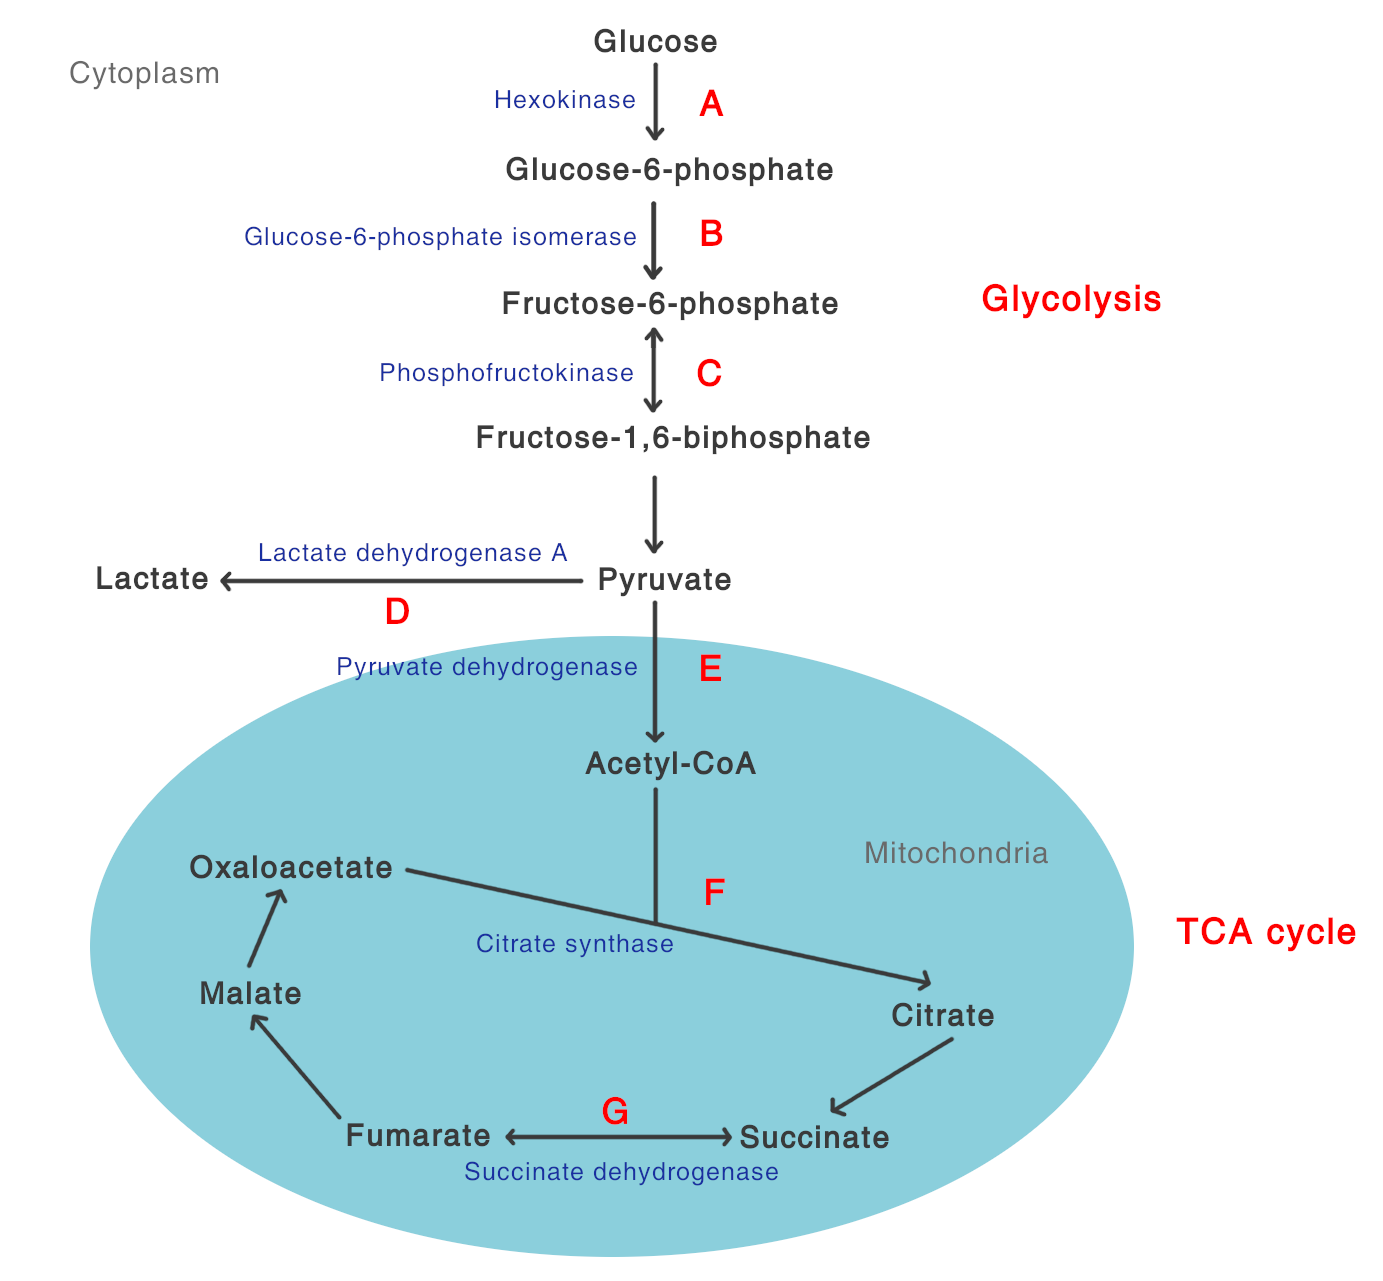
\includegraphics[scale=0.52]{fig9.png}
	\caption{\textbf{An overview of reactions involved in glycolysis and the TCA cycle.}
\\ Selected reactions for flux distribution analysis are marked in red. Important enzymes are marked in blue. 
}
\label{figure:9}
\end{figure}

\begin{figure}
\centering
	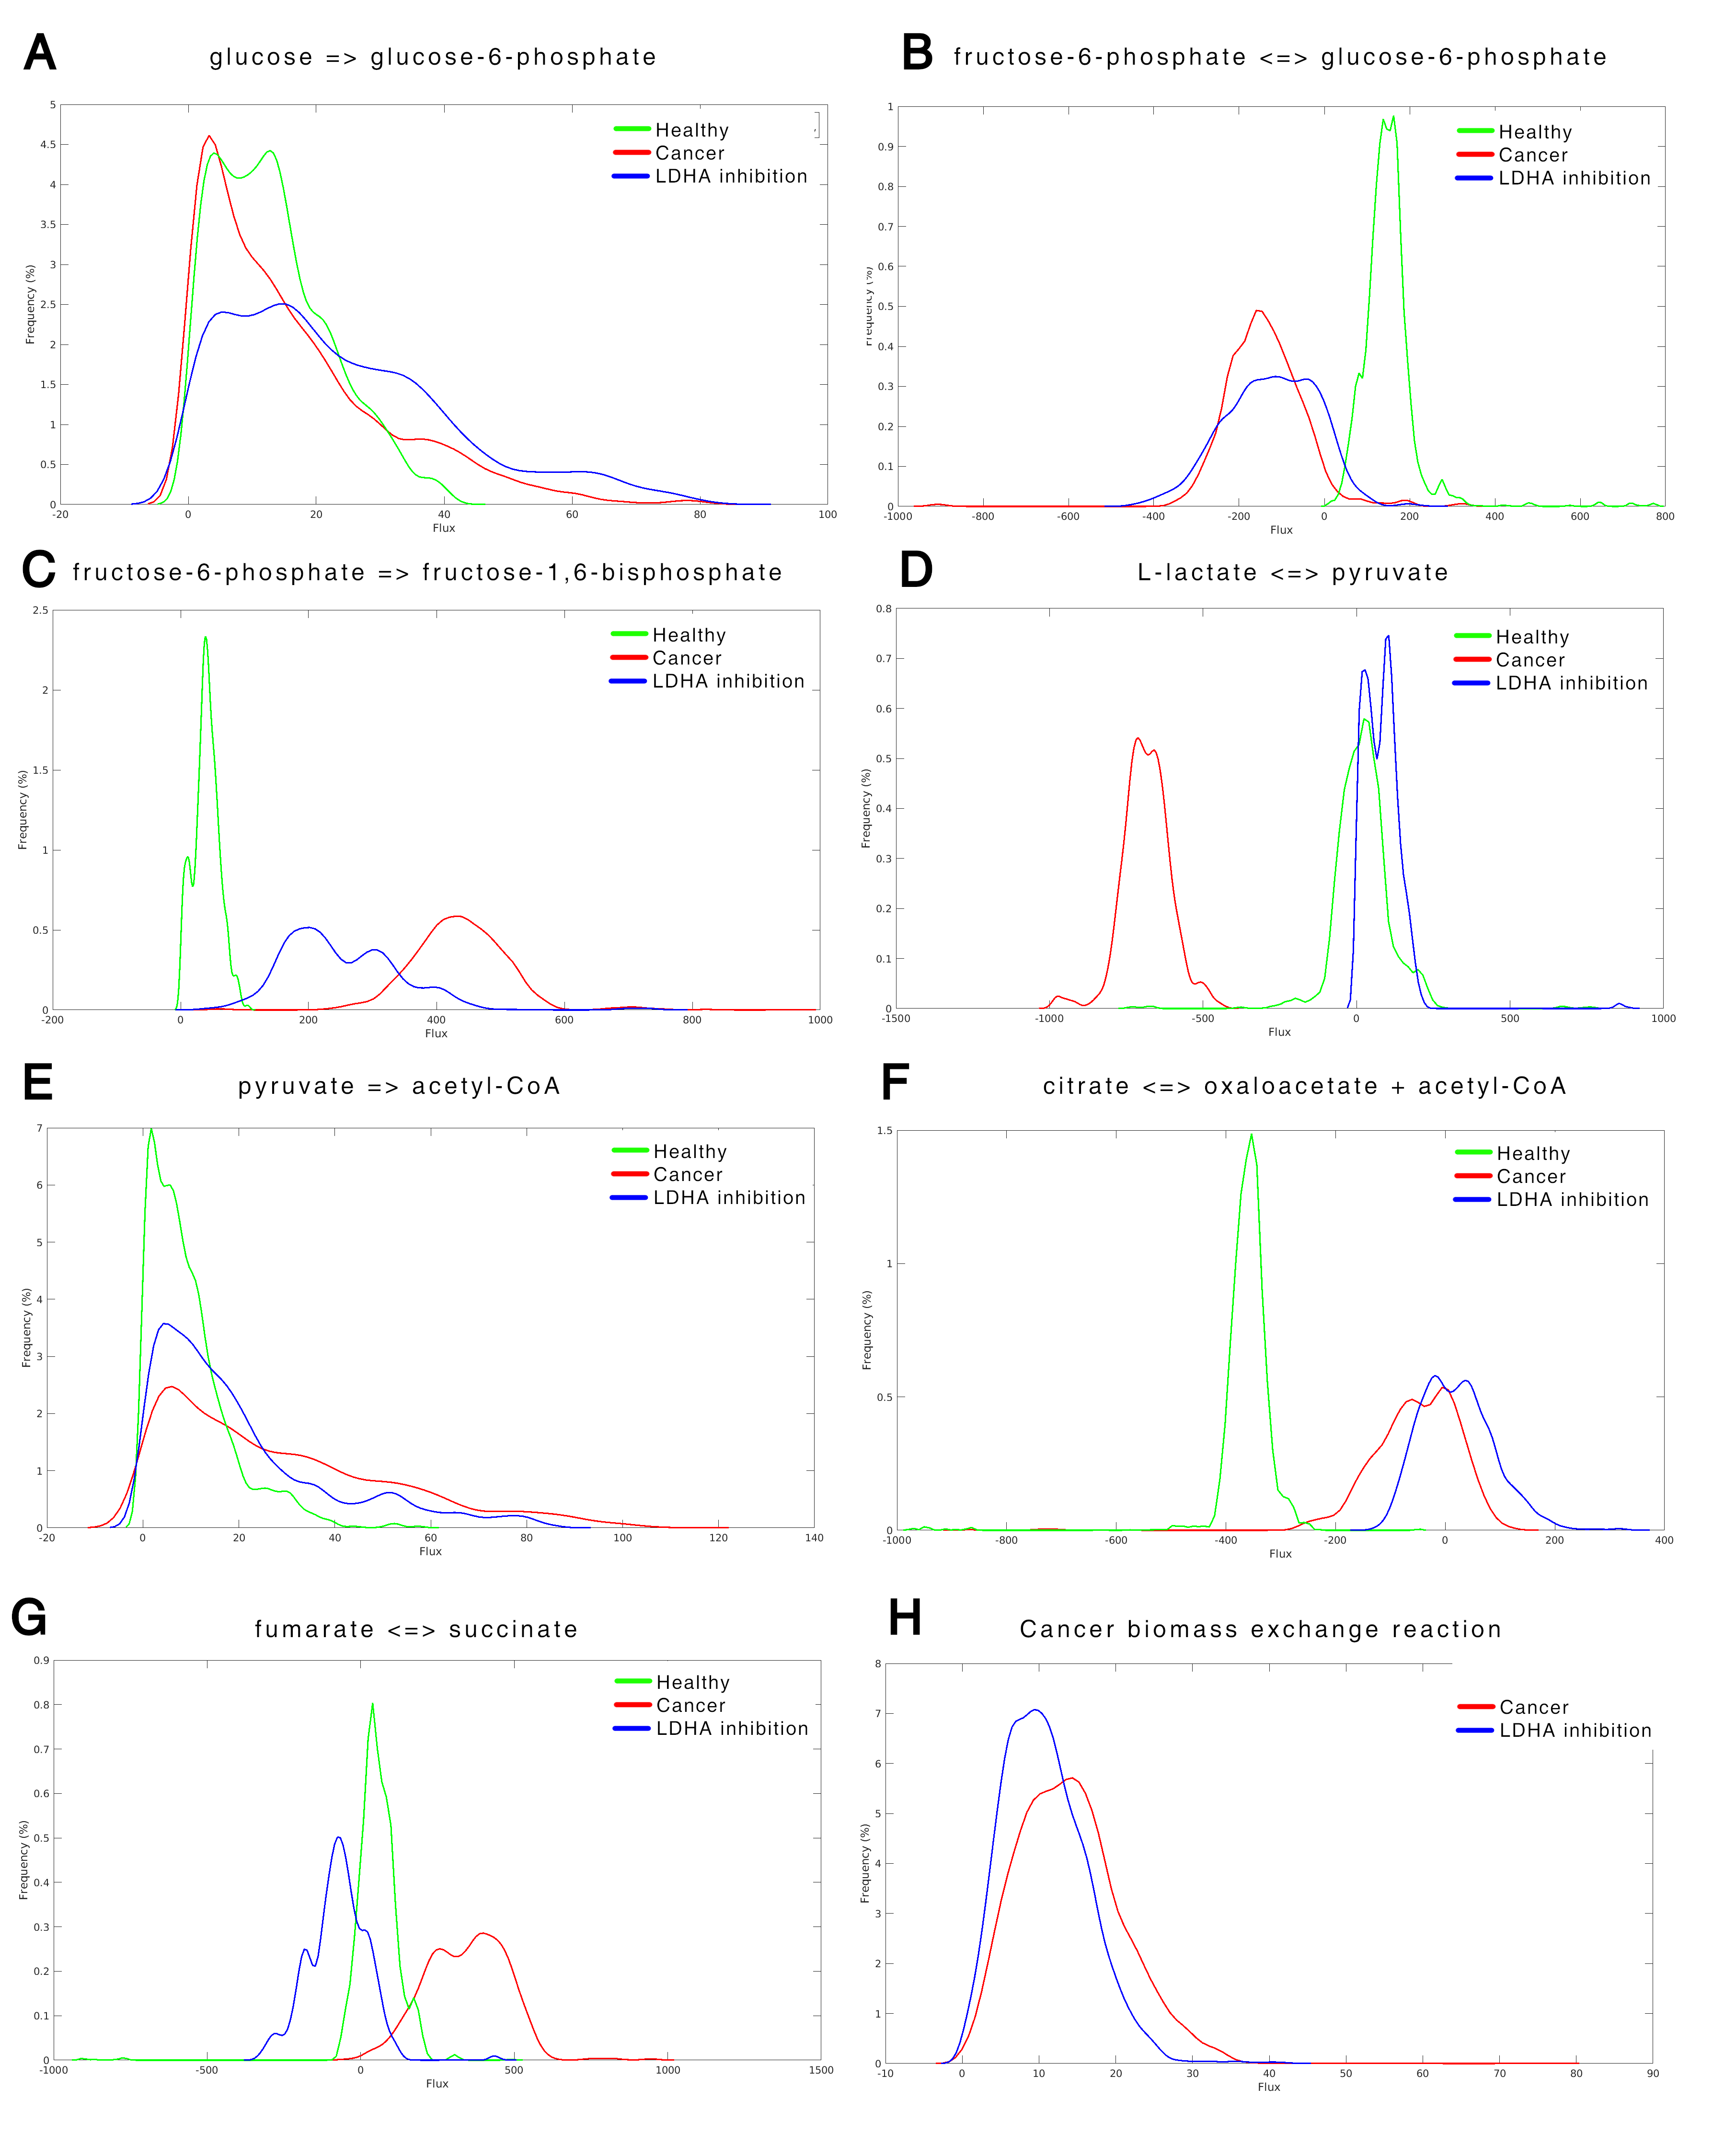
\includegraphics[scale=0.2]{fig10.png}
	\caption{\textbf{Flux probability distributions for the breast cancer, healthy breast cell and \textit{in silico} LDHA inhibition model $*$.}
	\\A, B, C) Reactions involved in glycolysis.
	\\D, E) Pyruvate reduction (D) and oxidation (E). 
	\\F, G) Reactions in the TCA cycle. 
	\\H) Cancer biomass objective function (not included in healthy breast cell model). 
\\$*$ Additional metabolites such as non-carbon containing metabolites are not shown in plot titles. 
}
\label{figure:10}
\end{figure}
% Can we change these to bar plots rather than distributions? 

\textbf{Glycolysis} \\
In comparison to the healthy model, the breast cancer model has a much larger flux through glycolysis. In reactions A, B and C the cancer model flux rates all increased in the direction of glycolysis, suggesting the glycolysis pathway is more active in breast cancer cells than healthy cells. The \textit{in silico} inhibition of LDHA appears to have little effect on the average flux rate in reactions A and B. This is could be because the glucose-6-phosphate and fructose-6-phosphate produced in these reactions can also be diverted into the pentose phosphate shunt and nucleotide synthesis, so they are less affected by inhibition of LDHA. The model with inhibited LDHA has a decreased flux rate, moving the mean flux closer to the healthy model levels. These results suggest that although inhibition of LDHA has some effect on the level of glycolysis occurring, LDHA inhibition alone isn’t enough to return the glycolysis pathway to that seen in a healthy cell phenotype.

\textbf{Pyruvate oxidation/reduction} \\
In reaction D, in the healthy model the flux distribution is roughly symmetric around zero, suggesting little flux occurs through this reaction under aerobic conditions. In cancer cells, the average flux is very negative, indicating a large amount of conversion to lactate even under aerobic conditions. This indicates the breast cancer model is demonstrating the Warburg effect and carrying out ‘aerobic glycolysis’. Inhibiting LDHA \textit{in silico} makes the reaction irreversible, preventing the reduction of pyruvate to lactate. Reaction E is the oxidation of pyruvate to acetyl-coenzyme A and the entrance into the TCA cycle. In cancer cells, the range of the flux distribution for reaction E is much greater than in the healthy cell and the average flux distribution is higher. This could be due to the higher rate of flux through through glycolysis in general. The LDHA inhibition model has a slightly decreased average flux in comparison to the cancer model, but the flux is not returned to levels as low as in the healthy cell. 

\textbf{TCA cycle} \\
Reactions F and G represent two conversions within the TCA cycle. In healthy cells where the TCA cycle is active, oxaloacetate and acetyl-coenzyme A react to produce citrate. However, in the cancer cell model, flux through this reaction is very low and the reaction is sometimes even reversed, favouring the break down of citrate. Unexpectedly, the inhibition of LHDA causes the further reversal of the this reaction. Reaction G shows the conversion of succinate to fumarate in the TCA cycle. As expected, the cancer model has a very low likelihood of flux in this direction, suggesting that the TCA cycle is not active in the cancer model. However, there is some flux through the reaction in this direction in the healthy model. Interestingly, the inhibition of LDHA further increases flux in the succinate to fumarate direction than the healthy model, suggesting that the TCA cycle is more active when LDHA inhibition model than in the healthy model. This could be due to the higher levels of pyruvate entering the TCA cycle in the LDHA inhibition model in comparison to the healthy model. 

\textbf{Cancer biomass} \\
The cancer biomass objective reaction totals the quantities of biomass contributing macromolecules such as lipids and proteins. The LDHA inhibition model appears to reduce the cancer biomass slightly, suggesting that this could lead to a decrease in cell proliferation and return to a metabolic profile more similar to a differentiated healthy cell. From the analysis of the 6 reactions involved in glycolysis and the TCA cycle, it is clear that inhibiting LDHA will have some effect on reducing the reliance on glycolysis and reactivating the TCA cycle. However, it is likely that there are multiple other pathways which are perturbed by this inhibition and that are contributing to this decreased cancer biomass. 

\subsection*{Application of uniform sampling to study a genome-scale metabolic networks - Lessons from an \textit{Arabidopsis thaliana} leaf metabolic model}

\subsubsection*{Using the OPTGP sampler to generate flux distributions of plant leaf metabolism}

The previously-published Arnold and Nikoloski (2014) metabolic model for \textit{Arabidopsis thaliana} leaf metabolism suits the purpose of a case study as it is manually curated, compartmentalized, mass-balanced, and obeys the law of conservation of energy. With its 407 metabolites and 549 reactions the model compiles to a recent knowledge base on confirmed metabolic reactions in the photosynthetic cells of \textit{A. thaliana}. Maximum biomass production, as defined by the authors was set as an objective function.

For sampling, the upper flux ($F_u$) and lower flux ($F_l$) of the objective function was set to the maximum possible value as calculated by FVA for optimal ($F_l\ \&\ F_u = F_{optimal}$) and near-optimal ($F_l\ \&\ F_u = 0.8\cdot F_{optimal}$) biomass production. Flux distributions of the conditions were compared as outlined below. Under both conditions the model dimension reduces to 547 reactions, excluding the other two biomass reactions previously implemented for varying carbon and nitrogen conditions. 

Here too the OPTGP sampler provides the best trade-off between run-time and convergence and was thus chosen to generate 100,000 samples in order to ensure convergence. Sample generation took 19min using OPTGP, far less than the estimated XX hours derived from a XXs step run-time and an assumed 5,000 sample convergence when using the CHRR sampler in MATLAB. 
%Is this actually true or should we be using CHRR here?? Lucy can you double check the XX numbers please 

\subsubsection*{Optimal and near-optimal objectives can result in vastly different flux distributions}
Flux sampling currently remains an underutilized technique across the plant sciences, with Gomes de Oliveira Dal’Molin \textit{et al.} (2015), who compared the flux distributions of passive and active transport of sucrose, glutamate and nitrate metabolites, being a rare example. Yet, by using sampling methods, rather than single FBA or FVA methods, biologically meaningful differences between conditions and imposed constraints can be analyzed in great detail. 

Imposing an objective function in order to constraint the flux space of the network induces an inherent observer bias on what the main cellular objective is under the defined metabolic environment. Maximum biomass production is generally considered as a primary cellular objective, especially in plants which are studied for their commercial value \cite{hay} \cite{schwender} \cite{grafahrend}. Recent literature however has highlighted that, in order to be able to efficiently respond to changing conditions, a more robust, slightly sub-optimal (near-optimal) biomass production defines biological reality\cite{schuetz}\cite{fischer}\cite{poolman}\cite{boyle}. Fischer and Sauer (2005), for example, used labeling across different \textit{Bacillus subtilis} mutants to show that wild-type biomass production is less than that of some mutants under optimal conditions, but that this sub-optimality is compensated by greater network robustness across changing environmental conditions and genetic perturbations. Later, Boyle \textit{et al.} (2017) demonstrated that maximum biomass and maximum ATP production in \textit{Chlamydomonas reinhardtii} are in part sacrificed for producing reducing equivalents in the form of oxaloacetate in the cytosol and plastids \cite{boyle}. 

Here, we use the Arnold and Nikoloski (2014) model to assess the differences in flux distributions of optimal and near-optimal biomass production of \textit{A. thaliana} leaves. Fig \ref{figure:ShowDistr} highlights some of the most prominent differences in distributions observed across the two set biomass optimalities. Different biomass solutions can have different biomass requirements: optimal biomass production has a higher probably requirement for CO$_2$ binding (Fig \ref{figure:ShowDistr} A), whereas near-optimal biomass production has a higher probable demand for ATP in the chloroplast (Fig \ref{figure:ShowDistr} B). This is likely due to the fact that near-optimal biomass production allows for significantly higher carbon storage (XX fold higher) in comparison to optimal biomass production, which is in agreement with findings from Boyle \textit{et al.} (2017). Transient carbon storage forms an integral part of photosynthetic tissues, where down-stream photosynthetic compounds like sugars and starch are accumulated during the day and consumed during the night. Figs \ref{figure:ShowDistr} C \& D effectively highlight how FVA cannot provide any information on the probability with which a given flux occurs within the solution space. While the assumption of a normal distribution within the FVA bounds holds true for C, it fails in D. Reactions which have the same FVA bounds can have very different flux probability distributions (Fig \ref{figure:ShowDistr} E) depending on the objective function. Multi-modality suggesting the existence of probably alternative flux solutions (Fig \ref{figure:ShowDistr} F) currently remain un-addressed in plant biology but could provide future explanations for understanding biological redundancy and no-effect mutations. These example effectively outline how the shape of the probability distributions, including, modality, skewness and kurtosis, capture features of the flux solutions space which cannot otherwise be explored using traditional FVA and FBA methods. 

\begin{figure}
\centering
	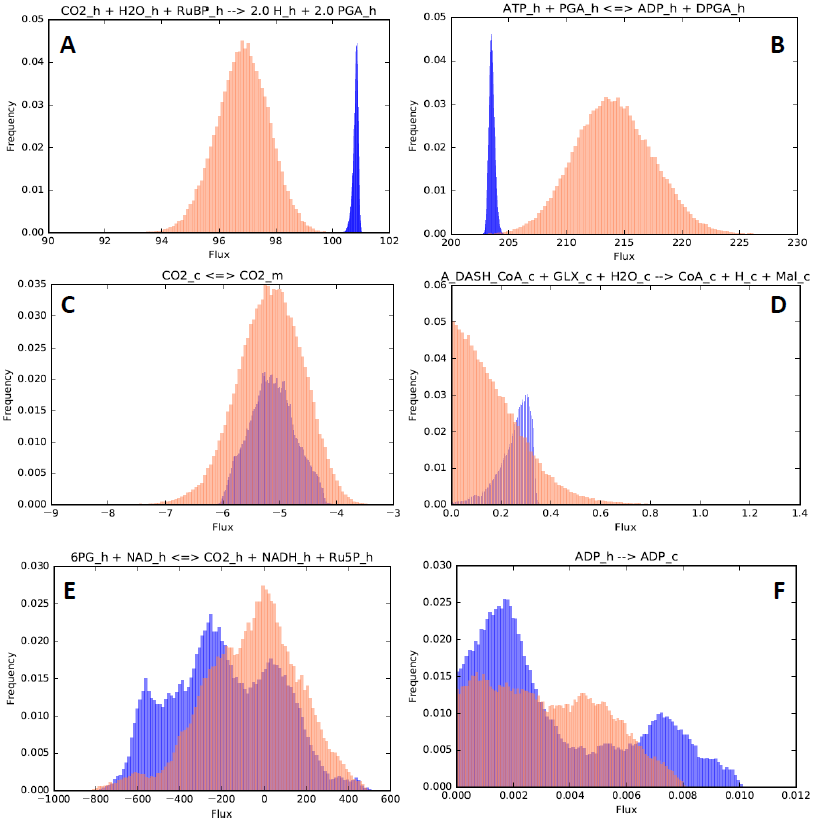
\includegraphics[scale=0.62]{ShowDistr.png}\\~\\
	\caption{\textbf{Example distributions highlighting probabilitistic differences of flux solutions of optimal and near-optimal biomass production in photosynthetic cells of \textit{A. thaliana}}
\\ Distributions where $F_l\ \&\ F_u = 0.8\cdot F_{optimal}$ are shown in red; distributions where $F_l\ \&\ F_u = F_{optimal}$ are shown in blue. 
}
\label{figure:ShowDistr}
\end{figure}

%Think of a better way of quantifying distribution shapes 
% think about calculating flux correlation to identify reactions of interest as in dal'molin paper? 
%look whether correlation coefficient analysis makes sense here?
%%%%%% The above might be more appropriate to explore for a further paper on plant metabolism 

\section*{Discussion}
Uniform sampling is an essential tool for studying the flux solution space of genome-scale metabolic reconstructions. Our work compares performance and usability of the three samplers available in the COBRApy and COBRA Toolbox. 

\subsection*{Difference in sampling steps to convergence}
This is the first study in which the number of sampling steps to convergence of ACHR, OPTGP and CHRR have been directly compared using a range of methods. Relying on a single method of assessing convergence is often flawed due to limitations associated with the techniques and tests\cite{Cowles}. Haraldsdottir \textit{et al.} (2017), which compared CHRR and ACHR, used a single method, the Gelman-Rubin diagnostic. Convergence was assumed when the Gelman-Rubin PSRF value was \textless{}1.1\cite{Haraldsdottir}. However, our results show that Gelman-Rubin PSRF values of \textless{}1.1 are often obtained before convergence \textbf{(Fig \ref{figure:4}B)}. In this project, in addition to the Gelman-Rubin PSRF, a range of methods including the running mean, XY deviation, and the Raftery \& Lewis convergence diagnostic were used. Each method used in this project gave a slightly different estimate of convergence at varying levels of precision, but they all clearly agreed that CHRR was less affected by dimensionality than ACHR and OPTGP. This result fits with the findings of Haraldsdottir \textit{et al.} (2017) and suggests that CHRR is better suited to sampling high dimension flux solution spaces than ACHR and OPTGP\cite{Haraldsdottir}. There was little difference between convergence in ACHR and OTPGP. Due to the time constraints, the largest models tested, \textit{T. maritima} and the human RBC, were not run for enough sampling steps to reach convergence on the ACHR and OPTGP samplers. Perhaps if the sampling had been continued it would have revealed more of a difference in convergence between the ACHR and OPTGP samplers. However, the number of sampling steps used is an improvement on other similar studies such as Megchelenbrink \textit{et al.} (2014), which was limited to 5,000 sampling steps\cite{Megchelenbrink}. 
%Bit of a dangerous thing to highlight in such detail that due to time-constraints we did not run the ACHR and OPTGP to convergence, reviewers will likely ask us to do this 

\subsection*{Run time in Python versus MATLAB}
The comparison of run times showed that the MATLAB implementation of CHRR was much slower than the two Python implementations, ACHR and OPTPG. Also, the MATLAB implementation of ACHR was much slower than the Python version, suggesting that the large difference in run time between CHRR and the other samplers is due to the differences between MATLAB and Python libraries, as opposed to the sampling algorithms used. The long run time per step of the CHRR sampler makes it impractical to use with large genome-scale metabolic models such as the breast cancer model (775 dimensions). A Python implementation of CHRR could improve run time per step to above that of OPTGP. In addition to the fast run time, CHRR converges more quickly, so it’s likely that a Python implementation would outperform OPTGP when comparing the run time to convergence.  

\subsection*{Differences in flux probability distributions}
The flux probability distributions produced by the three samplers have not previously been compared. Megchelenbrink \textit{et al.} (2014), which compared OPTGP to the generalized parallel sampler, found there were significant differences in the flux probability distributions produced and concluded convergence of the generalized parallel sampler to a non-uniform distribution \cite{Megchelenbrink}. Here, multiple methods were used to identify differences between the flux probability distributions. We did not not find any significantly different flux probability distributions produced between samplers and no evidence of non-uniform convergence was found. The only consistent difference observed was in the two larger models, \textit{T. maritima} and the human RBC, which were run to sample step counts below convergence. It was found that at high or low normalized means, CHRR produced a slightly different mean flux value than ACHR and OPTPG. This result has not been reported previously and suggests that CHRR is perhaps oversampling the flux values near the constraints of the flux solution space. Alternatively, ACHR and OPTGP could be oversampling the centre of the flux solution space due to the artificial centering step used in the algorithm. As these results were observed below convergence (20,000 sampling steps), it is possible that these differences are due to the ACHR and OPTGP samplers not yet having reached a stationary uniform distribution. Future studies could investigate this by running the ACHR and OPTGP samplers for longer to see if these differences persist at convergence. 

Despite observing differences between the samplers, it is impossible to say which sampler was closer to the true flux probability distribution, as this is unknown. Further research could aim to determine the exact flux solution space of a simple toy model using mathematical methods, such as convex analysis and vertex enumeration\cite{Schellenberger}, and then use this to compare the performance of the samplers.

\subsection*{Which sampler should computational biologists choose?}
The most impactful differences observed between the three samplers was the number of sampling steps to convergence and run time per sampling step. Both these features are linked to the overall useability of the algorithms as they impact the final run time of the algorithm. Although the number of sampling steps needed for ACHR and OPTGP convergence is higher, they have a much faster run time per step. In comparison, CHRR seems to converge at below 5,000 sampling steps for models with dimensions up to 1000, but has a very slow run time per step. 

The best performing sampler therefore depends on the intended application. If the research involves changing multiple constraints of the model, for example to simulate gene knockouts or environmental effects, a sampler with a shorter run time might be beneficial. Additionally, when working with smaller less complex models, the CHRR sampler run time is still fairly short and won’t make a large practical difference to the research. For example, for the \textit{E coli} core model (24 dimensions), the difference in time between running CHRR and OPTGP to convergence is around 14 minutes. In comparison, when working with high dimension models, such as the breast cancer cell model and the \textit{A. thaliana} leaf model, the run time per step is vastly different. Running the breast cancer cell model for just 5,000 iterations on CHRR would take 442 hours more than OPTGP, increasing the run time to impractical levels for most studies. Given that flux sampling is preferentially applied to large metabolic networks since this is where it's steady-state assumption outweighs the requirement for kinetic parameters, OPTGP should be a likely choice for most biologists. 

For our case study analyses, OPTGP was chosen as the most suitable sampler as it has a faster run time per sampling step than CHRR and likely converges at a lower step count than ACHR. The COBRApy package allowed the breast cancer and healthy model flux distributions to be compared and also enabled the simulation of LDHA inhibition through changing the lower flux bound of the pyruvate to lactate reversible reaction. Use of uniform sampling allowed comparisons of the underlying probability distributions, providing more information than FBA or FVA. While near-optimal to optimal biomass production was set as the objective for all breast cell models, optimal and near-optimal conditions were compared using the \textit{A. thaliana} model. Our results effectively demonstrate that slight changes in optimality can significantly alter flux distributions affecting their, modality, kurtosis, and skewness. 

Evidently, the level of accuracy of the flux probability distribution is an important factor when deciding on a sampler to use. Some applications of FBA may require less precise estimates of flux values. For example, in the breast cancer cell application which investigating the effects of LDHA inhibition, the accuracy required was low as the differences between the flux distributions in the three models being tested were large and the results were mainly being used qualitatively. Therefore, sampling below convergence is allowable and OPTGP was the best choice due to the fast run time per step. For the \textit{A. thaliana} leaf model, on the other hand, 100,000 samples were ran in order to ensure convergence. Since the results were used to detect differences in the sampling distributions of optimal and near-optimal biomass production, a higher accuracy is required in order to achieve completely uniform and stationary distribution. OPTGP is still the better choice here since running it's run-time advantage outperforms the time to convergence. 
%Need to re-write this if we end up using the CHRR for the Arabidopsis model

The final consideration for choosing a sampler is usability. The COBRApy and COBRA Toolbox have very similar functionalities so the major difference between them is the use of MATLAB versus Python. Unlike Python, MATLAB is not open-source and requires a license fee. A separate installation of a linear programming solver also complicates the installation and setup process of the COBRA Toolbox for non-expert users. Python is a much more popular language, especially within the field of bioinformaticians, so the ACHR and OPTGP implementations may be much easier for the majority of users to setup and use within existing workflows.

Future research into why the CHRR sampler convergence is not affected by the flux solutions space dimensions would be of interest and could potentially aid in the design of even better performing, faster samplers. This could perhaps involve further investigation into the algorithms movement around the flux solution space.

More investigation into the differences in distributions between the three samplers could help explain the finding that CHRR produced a different mean flux value than ACHR and OPTGP when sampling reactions with high or low normalized mean flux values. Further methods of comparing the distribution such as looking at the most common flux value range, the interquartile range and range would provide more information and identify more patterns. 

We focused on uniform sampling Monte Carlo methods provided by COBRApy and the COBRA Toolbox, which are the most widely used in the field. Further work could expand the evaluation to algorithms available such as ll-ACHRB (loopless Artificially Centered Hit-and-Run on a Box)\cite{Saa} and the poling-based flux balance analysis\cite{Binns}. 

\section*{Conclusion}
Our results successfully evaluated the performance of three uniform samplers in estimating the flux probability distribution of genome-scale metabolic models. CHRR was found to have the fewest sampling steps to convergence and also was not affected by increasing dimensionality of the flux solution space, making it a good choice for sampling high dimensional networks to convergence. OPTGP and ACHR took more sampling steps to reach convergence but the Python implementations of these algorithms were much faster than CHRR. CHRR was found to have a very slow run time per step when sampling high dimension flux solution spaces, potentially making it impractical for use in some applications.

These findings will aid computational biologists in choosing the best performing and most efficient sampler from the popular COBRApy package and COBRA Toolbox. The choice of sampler should be informed by the complexity and size of the metabolic model and the desired accuracy of the resulting flux probability distributions. The performance of the sampler is dependent on the intended application. Additionally, assessment of convergence of the sampling chains can be complex and time consuming, so estimations of the number of sampling steps to convergence found in this project can be used to inform experimental design of future flux sampling studies. 

Future work will continue to explore the small differences observed between the flux probability distributions produced by the samplers. In addition, the behaviour of the algorithms should be further investigated to understand why CHRR converges in fewer steps than the other two algorithms. The findings indicate that a Python implementation of CHRR would greatly outperform the existing samplers available in COBRA. The development of a Python implementation would therefore be very beneficial to researchers using FBA, especially those studying high dimension models such as reconstructions of the human metabolism. Ultimately, this will increase the potential for application of FBA for analysis of genome-scale metabolic models and could further improve our understanding of the metabolism at the scale of the organism. 


%\section*{Supporting information}

% Include only the SI item label in the paragraph heading. Use the \nameref{label} command to cite SI items in the text.
% \paragraph*{S1 Fig.}
% \label{S1_Fig}
% {\bf Bold the title sentence.} Add descriptive text after the title of the item (optional).

% \paragraph*{S1 Appendix.}
% \label{S1_Appendix}
% {\bf Lorem ipsum.} Maecenas convallis mauris sit amet sem ultrices gravida. Etiam eget sapien nibh. Sed ac ipsum eget enim egestas ullamcorper nec euismod ligula. Curabitur fringilla pulvinar lectus consectetur pellentesque.

% \paragraph*{S1 Table.}
% \label{S1_Table}
% {\bf Lorem ipsum.} Maecenas convallis mauris sit amet sem ultrices gravida. Etiam eget sapien nibh. Sed ac ipsum eget enim egestas ullamcorper nec euismod ligula. Curabitur fringilla pulvinar lectus consectetur pellentesque.

\section*{Acknowledgments}
% Not sure what to write here, do we need to acknowledge BBSRC? 

\nolinenumbers

\bibliography{rp2}
\bibliographystyle{plos2015}


\end{document}

% Place tables after the first paragraph in which they are cited.
% \begin{table}[!ht]
% \begin{adjustwidth}{-2.25in}{0in} % Comment out/remove adjustwidth environment if table fits in text column.
% \centering
% \caption{
% {\bf Table caption Nulla mi mi, venenatis sed ipsum varius, volutpat euismod diam.}}
% \begin{tabular}{|l+l|l|l|l|l|l|l|}
% \hline
% \multicolumn{4}{|l|}{\bf Heading1} & \multicolumn{4}{|l|}{\bf Heading2}\\ \thickhline
% $cell1 row1$ & cell2 row 1 & cell3 row 1 & cell4 row 1 & cell5 row 1 & cell6 row 1 & cell7 row 1 & cell8 row 1\\ \hline
% $cell1 row2$ & cell2 row 2 & cell3 row 2 & cell4 row 2 & cell5 row 2 & cell6 row 2 & cell7 row 2 & cell8 row 2\\ \hline
% $cell1 row3$ & cell2 row 3 & cell3 row 3 & cell4 row 3 & cell5 row 3 & cell6 row 3 & cell7 row 3 & cell8 row 3\\ \hline
% \end{tabular}
% \begin{flushleft} Table notes Phasellus venenatis, tortor nec vestibulum mattis, massa tortor interdum felis, nec pellentesque metus tortor nec nisl. Ut ornare mauris tellus, vel dapibus arcu suscipit sed.
% \end{flushleft}
% \label{table1}
% \end{adjustwidth}
% \end{table}


% % For figure citations, please use "Fig" instead of "Figure".

% % Place figure captions after the first paragraph in which they are cited.
% % \begin{figure}[!h]
% % \caption{{\bf Bold the figure title.}
% % Figure caption text here, please use this space for the figure panel descriptions instead of using subfigure commands. A: Lorem ipsum dolor sit amet. B: Consectetur adipiscing elit.}
% % \label{fig1}
% % \end{figure}


